% Chapter 2
\chapter{Results} % Main chapter title
\label{Chapter5} % For referencing the chapter elsewhere, use \ref{Chapter2} 
\minitoc
%----------------------------------------------------------------------------------------

%% Define some commands to keep the formatting separated from the content 
%\newcommand{\keyword}[1]{\textbf{#1}}
%\newcommand{\tabhead}[1]{\textbf{#1}}
%\newcommand{\code}[1]{\texttt{#1}}
%\newcommand{\file}[1]{\texttt{\bfseries#1}}
%\newcommand{\option}[1]{\texttt{\itshape#1}}

%----------------------------------------------------------------------------------------

This chapter presents the results of each evaluated model (i.e. \textit{GaHMM profile, seasonal and interactional}). The evaluation information, expossed in section \ref{sec:eval_all}, is used in conjuction with the results of each model in a study case where we compare the Noth-East and South-West ventilation systems. Furthermore, one practical application is proposed for the \textit{GaHMM} profile model. In the penultimate section, we include a comparison of our proposition (i.e. \textit{GaHMM profile model}) against \textit{DayFilter} approach that is considered as one of the state of art for AFDD \cite{kim2017review,miller2015automated}. At the end of this chapter, we include the feedback   from building control system specialists of Synergy BTC AG.

\section{Results}

\subsection{Results of the GaHMM seasonal model}
\label{sec:seasonal_results}

As it was explained in section \ref{sec:seasonal_evaluation}, we can evaluate a \textit{GaHMM seasonal} model by using the log probability of $p(\mathbb{O}|\lambda)$, average of $p(\mathbb{O}|\mathbb{S})$ and PCA visualization. 
Here we indicate how the clusters of \textit{summer, winter, coldest transition and hottest transition} are distributed across years. In addition, we consider it interesting to add to the $S_{vector}$ the \textit{sunshine presence} variable \footnote{Finally, precipitation measures were not added because they present so many $nan$ values that causes a bad monthly distribution.}. The final model (including sunshine presence variable) with 6 features achieves an average of $p(\mathbb{O}|\mathbb{S}) = 0.992624$ which is still good, similar to the results presented in table \ref{tab:result_training_seasonal}. The clusters are distributed over the whole timeline in this way: \textit{winter} $= 26.9$, \textit{summer} $=21.0$, \textit{coldest transition} $=29.1$, \textit{hottest transition} $=23.0$. Each one has its own particular monthly distribution as one can see in figure \ref{fig:monthly}. For example, winter is distributed over $[Oct, Nov, Dec, Jan, Feb, Mar]$ in this manner $[2\%, 19.5\%, 22.5\%, 24.5\%, 19.5\%, 8\%, 4\%]$.   


\begin{figure}[h!]
  \vspace{0.5em} %better style
  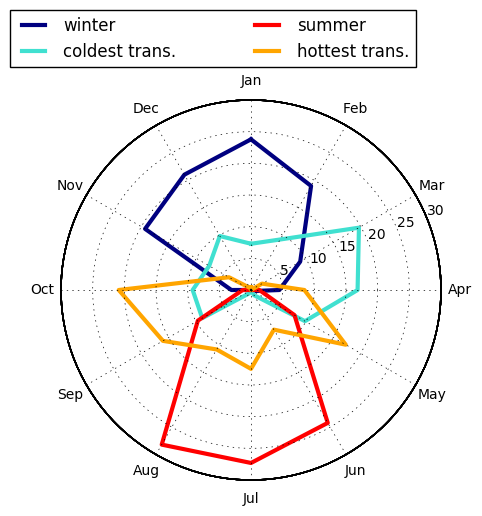
\includegraphics[scale=0.65]{Figures/Monthly_distribution.jpg}
  \caption{Monthly distribution for clusters: \textit{summer, winter, hottest and coldest transition}. $S_{vector}$ contains variables outdoor temperature, weather temperature and sunshine presence.}
  \label{fig:monthly}
\end{figure} 


Something to note is how the spring and autumn period share some patterns in common, this is the case when the \textit{hottest transition} appears in May or when the \textit{coldest transition} appears in October for instance. Other interesting aspects is how the coldest and hottest transitions remain inside of the winter and summer period respectively. One can also see how these clusters are distributed in a daily fashion in Figure \ref{fig:daily}, one observes that each cluster is distributed in an equitable fashion over \textbf{a)} working days, weekends and holidays; and \textbf{b)} the days of the week in general.   

\begin{figure}[h!]
  \vspace{0.5em} %better style
  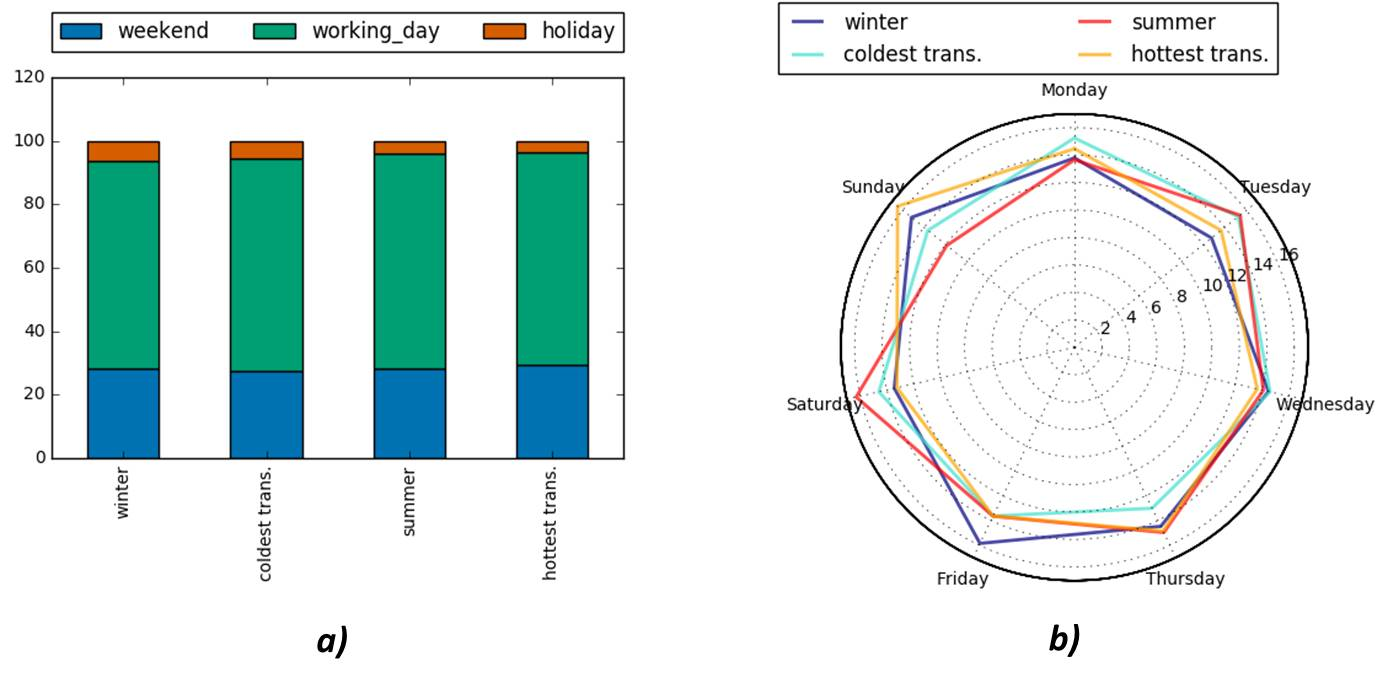
\includegraphics[scale=0.65]{Figures/daily_distribution_season.jpg}
  \caption{Monthly distribution for clusters: \textit{summer, winter, hottest and coldest transition}. $S_{vector}$ contains variables outdoor temperature, weather temperature and sunshine presence.}
  \label{fig:daily}
\end{figure} 

Finally, a calendar visualization is proposed to see the distribution of these clusters. Annex \ref{fig:s_vector_temperature} contains a calendar visualization for \textbf{a)} $S_{vector}$ using outdoor temperature and weather temperature; and \textbf{b)} $S_{vector}$ using outdoor temperature, weather temperature and sunshine presence. The sunshine presence variable affects the clustering such that they become more heterogeneous and blended being in this way a more representative abstraction of the weather nature.  

\begin{figure}[h!]
  \vspace{0.5em} %better style
  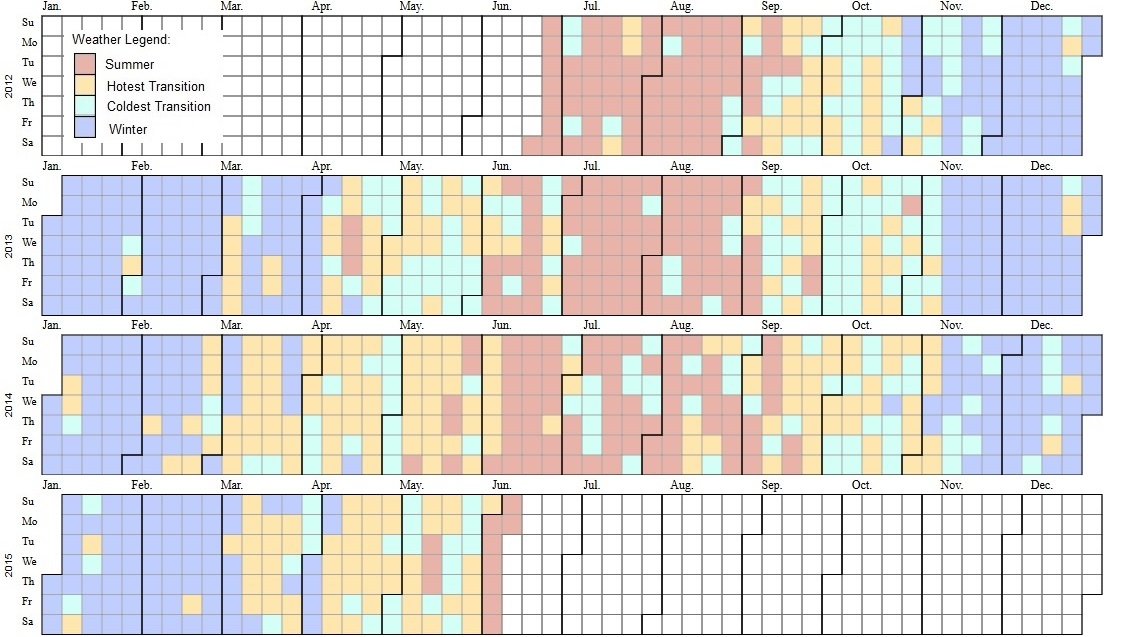
\includegraphics[scale=0.45]{Figures/temperatures.jpg}
  \caption{\textbf{a)} Daily representation of clusters: \textit{summer, winter, coldest and hottest transition} using a $S_{vector}$ with outdoor temperature and weather temperature.}
  \label{fig:s_vector_temperature}
\end{figure}

\begin{figure}[h!]
  \vspace{0.5em} %better style
  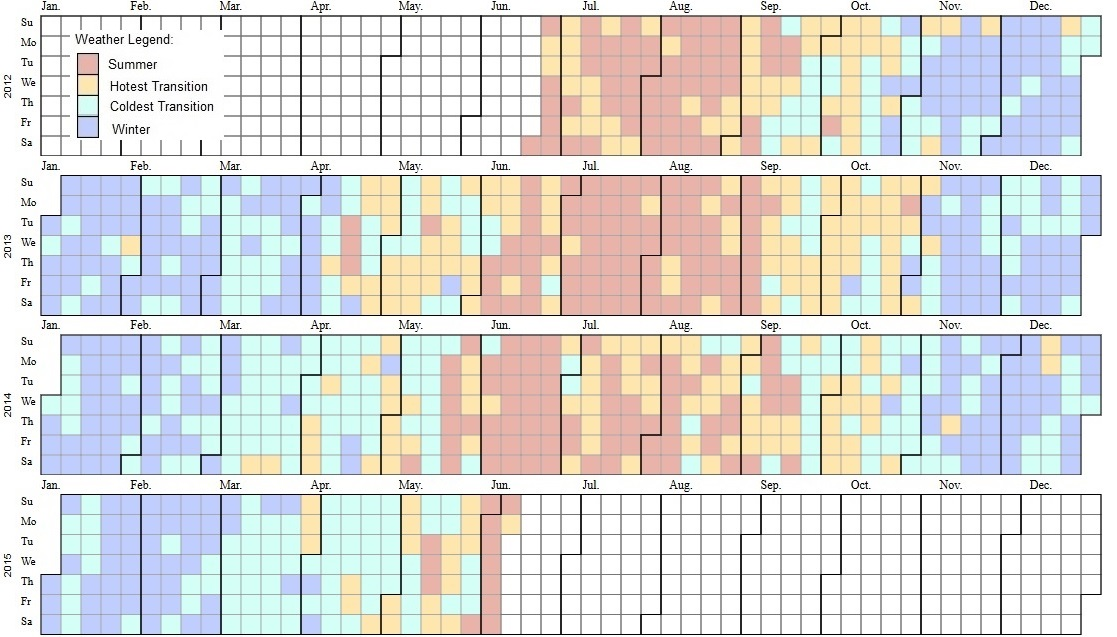
\includegraphics[scale=0.45]{Figures/sushine.jpg}
  \caption{\textbf{b)} Daily representation of clusters: \textit{summer, winter, coldest and hottest transition} using a $S_{vector}$ with outdoor temperature, weather temperature and sunshine presence variables.}
  \label{fig:s_vector_sunshine}
\end{figure}




%--------------------------------------------------------------------------------------
\subsection{Results of the GaHMM interactional model}
\label{sec:interactional_results}

As it was exposed in section \ref{sec:interactional_evaluation}, three clusters were found by using the best \textit{GaHMM} interactional model. In this model, the $R_{vector}$ represents the existing correlation between categories \textit{[A\_3, A\_{4\_1}, A\_{4\_2},  A\_{6\_1}, A\_{6\_2}]} and the $CO_2$ levels of the North-East part of the building. Following this idea, \textbf{Regimen of Negative Correlation} contains a collection of days where the negative correlation in the $R_{vector}$ is relevant. \textbf{Regimen of Weak Correlation} contains a collection of days where there is a weak linear correlation in the $R_{vector}$, and finally, \textbf{Regimen of Positive Correlation} contains a collection of days where \textbf{$R_{vector}$} has mostly positive correlation. Each center of the cluster is represented by the mean vector and a standard deviation (see table \ref{tab:regimen_centers}). For example, one reads that the $CO_2$ levels has, in average, a correlation of -0.6 with the angles of the North exterior blinds in Regimen of Negative Correlation.

% Table generated by Excel2LaTeX from sheet 'Hoja1'
\begin{table}[htbp]
  \centering
  \tiny
  \caption{Center vector of clusters: \textit{[Regimen of Negative Correlation, Positive Correlation and Weak correlation]} with their correspondent standard deviation.}
    \begin{tabular}{|l|c|c|c|c|c|}
    \multicolumn{6}{c}{\textcolor[rgb]{ .31,  .506,  .741}{\textbf{Regimen of Negative Correlation}}} \bigstrut[b]\\
    \hline
    \textbf{CO2 vs.} & \multicolumn{1}{l|}{\textbf{Blinds angle N Out}} & \multicolumn{1}{l|}{\textbf{ Blinds angle N In}} & \multicolumn{1}{l|}{\textbf{ Blinds angle E Out}} & \multicolumn{1}{l|}{\textbf{Blinds angle E In}} & \multicolumn{1}{l|}{\textbf{Blinds height N Out}} \bigstrut\\
    \hline
    \textit{mean\_vector} & -0.60 & -0.50 & -0.50 & -0.60 & -0.60 \bigstrut\\
    \hline
    \textit{std} & 0.10 & 0.17 & 0.14 & 0.10 & 0.10 \bigstrut\\
    \hline
    \textbf{CO2 vs.} & \multicolumn{1}{l|}{\textbf{Blinds height N In}} & \multicolumn{1}{l|}{\textbf{ Blinds height E Out}} & \multicolumn{1}{l|}{\textbf{Blinds height E In}} & \multicolumn{1}{l|}{\textbf{Temp. Vent. NE Out}} & \multicolumn{1}{l|}{\textbf{Temp. Vent. NE In}} \bigstrut\\
    \hline
    \textit{mean} & -0.60 & -0.10 & -0.30 & 0.70 & 0.10 \bigstrut\\
    \hline
    \textit{std} & 0.10 & 0.37 & 0.22 & 0.20 & 0.50 \bigstrut\\
    \hline
    \multicolumn{1}{l}{} & \multicolumn{1}{c}{} & \multicolumn{1}{c}{} & \multicolumn{1}{c}{} & \multicolumn{1}{c}{} & \multicolumn{1}{c}{} \bigstrut[t]\\
    \multicolumn{6}{c}{\textcolor[rgb]{ .31,  .506,  .741}{\textbf{Regimen of Positive Correlation}}} \bigstrut[b]\\
    \hline
    \textbf{CO2 vs.} & \multicolumn{1}{l|}{\textbf{Blinds angle N Out}} & \multicolumn{1}{l|}{\textbf{ Blinds angle N In}} & \multicolumn{1}{l|}{\textbf{ Blinds angle E Out}} & \multicolumn{1}{l|}{\textbf{Blinds angle E In}} & \multicolumn{1}{l|}{\textbf{Blinds height N Out}} \bigstrut\\
    \hline
    \textit{mean} & 0.50 & 0.50 & 0.50 & 0.50 & 0.50 \bigstrut\\
    \hline
    \textit{std} & 0.20 & 0.20 & 0.17 & 0.20 & 0.20 \bigstrut\\
    \hline
    \textbf{CO2 vs.} & \multicolumn{1}{l|}{\textbf{Blinds height N In}} & \multicolumn{1}{l|}{\textbf{ Blinds height E Out}} & \multicolumn{1}{l|}{\textbf{Blinds height E In}} & \multicolumn{1}{l|}{\textbf{Temp. Vent. NE Out}} & \multicolumn{1}{l|}{\textbf{Temp. Vent. NE In}} \bigstrut\\
    \hline
    \textit{mean} & 0.50 & 0.40 & 0.50 & 0.40 & 0.30 \bigstrut\\
    \hline
    \textit{std} & 0.20 & 0.22 & 0.17 & 0.62 & 0.67 \bigstrut\\
    \hline
    \multicolumn{1}{l}{} & \multicolumn{1}{c}{} & \multicolumn{1}{c}{} & \multicolumn{1}{c}{} & \multicolumn{1}{c}{} & \multicolumn{1}{c}{} \bigstrut[t]\\
    \multicolumn{6}{c}{\textcolor[rgb]{ .31,  .506,  .741}{\textbf{Regimen of Weak Correlation}}} \bigstrut[b]\\
    \hline
    \textbf{CO2 vs.} & \multicolumn{1}{l|}{Blinds angle N Out} & \multicolumn{1}{l|}{ Blinds angle N In} & \multicolumn{1}{l|}{ Blinds angle E Out} & \multicolumn{1}{l|}{Blinds angle E In} & \multicolumn{1}{l|}{Blinds height N Out} \bigstrut\\
    \hline
    mean & -0.10 & 0.00 & -0.20 & -0.10 & -0.10 \bigstrut\\
    \hline
    std & 0.00 & 0.00 & 0.00 & 0.00 & 0.00 \bigstrut\\
    \hline
    \textbf{CO2 vs.} & \multicolumn{1}{l|}{Blinds height N In} & \multicolumn{1}{l|}{ Blinds height E Out} & \multicolumn{1}{l|}{Blinds height E In} & \multicolumn{1}{l|}{Temp. Vent. NE Out} & \multicolumn{1}{l|}{Temp. Vent. NE In} \bigstrut\\
    \hline
    \textit{mean} & -0.10 & 0.10 & -0.10 & 0.20 & 0.30 \bigstrut\\
    \hline
    \textit{std} & 0    & 0    & 0    & 0    & 0 \bigstrut\\
    \hline
    \end{tabular}%
  \label{tab:regimen_centers}%
\end{table}%

Clusters of Regimen of Negative, Weak and Positive correlation are distributed over the complete timeline (i.e. 1801 days) in the following respective manner $63.8\%, 28.2\%, 8\%$. Each cluster has a dominant component (see figure \ref{fig:daily_distribution} and \ref{fig:r_distribution}). For example, the regimen of Negative correlation is formed by 631 ($93.07\%$) working days, 26 ($3.83\%$) weekend days and 21 ($3.10\%$) holidays. Clearly, this cluster describes the interrelation of variables when there is occupant presence. In contrast, the regimen of Weak Correlation has a dominant component of weekend days (199 days) where generally there is absence of occupant presence. Thus one can associate a weak correlation with absence of occupants. However, there are cases where the correlation is weak, even if there are occupants present \footnote{Occupant presence assumed because the $CO_2$ levels follows the typical profile $ ID=[12, 15, 16] $ annex \ref{cluster_profiles}, for instance.}, this is the yellow area in figure \ref{fig:r_distribution}. \\

We conclude a weak correlation implies absence of occupants but at the same time is an indicative (in the case when there is actual occupant presence) of an atypical interaction of variables, that could involve cases where the blinds are not at all used during the day (totally closed for instance) or the exhaust air temperature stays static during the entire day, or other atypical situations (it could imply sensor faults). Unfortunately, we do not have a ground truth information for these nonconforming days, and therefore we cannot corroborate this hypothesis. Nevertheless when one sees the details of this cluster, one observes time periods where the correlation is weak for business days. One example, is the period of \textit{Friday November $8^{th}$, 2013} to \textit{Tuesday November $12^{th}$, 2013} that presents frozen data in all the variables of the dataset (see figure \ref{fig:maintenance}). We suppose it corresponds to a building maintenance period. Finally, the Positive correlation has a dominant component of Saturdays, this correspond to days where the $CO_2$ levels were accumulated until Friday ($CO_2$ levels in the range of 800 ppm at midnight), and on Saturday the $CO_2$ levels diminish during the day (see profile $ID=26$, annex \ref{cluster_profiles}). All the information in this section is used in the case study in section \ref{section:case_study_1}. 

\begin{figure}[h!]
  \vspace{0.5em} %better style
  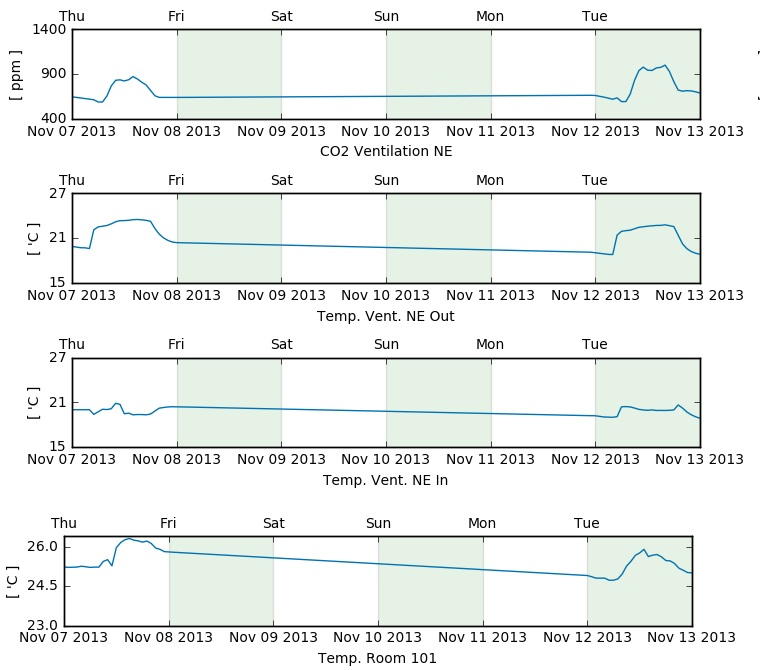
\includegraphics[scale=0.65]{Figures/maintenance_period.jpg}
  \caption{Discovered building maintenance period: frozen data in all the variables of the dataset.}
  \label{fig:maintenance}
\end{figure}



\begin{figure}[h!]
  \vspace{0.5em} %better style
  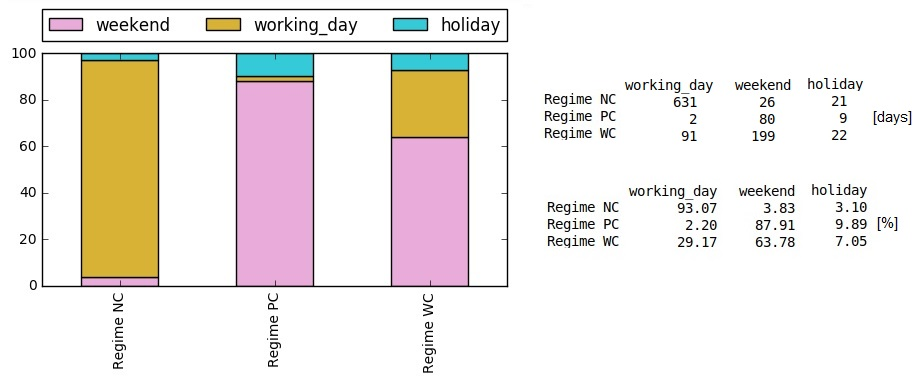
\includegraphics[scale=0.65]{Figures/Distribution_daily.jpg}
  \caption{Distribution for clusters: \textit{Regimen of Negative, Weak and Positive correlation} over working days, weekends and holidays.}
  \label{fig:daily_distribution}
\end{figure}


\begin{figure}[h!]
  \vspace{0.5em} %better style
  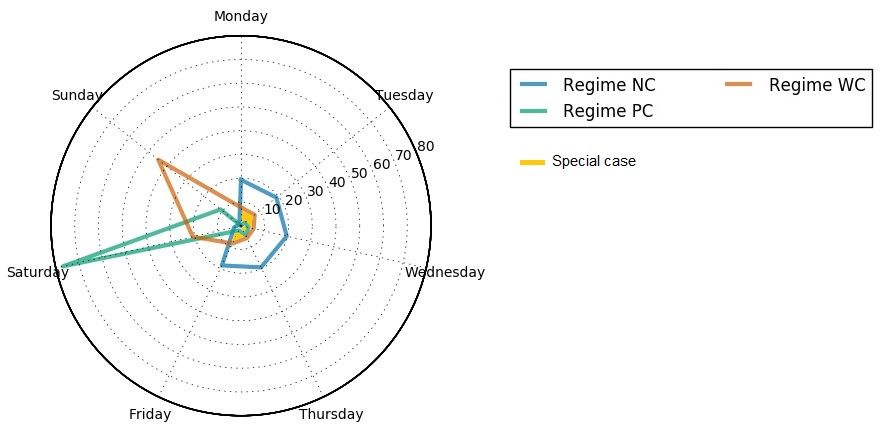
\includegraphics[scale=0.65]{Figures/Interactional_cluster_daily_distribution.jpg}
  \caption{Distribution for clusters: \textit{Regimen of Negative, Weak and Positive correlation} over working days, weekends and holidays.}
  \label{fig:r_distribution}
\end{figure}


%--------------------------------------------------------------------------------------
\subsection{Results of the GaHMM profile model}
\label{sec:profile_results}

Each variable has his own \textit{GaHMM profile model} and their results are in the digital folder annex: \textit{iPythonBooks/Diversity of profiles}. To exemplify the results of the \textit{GaHMM profile} model, we propose to use the $CO_2$ levels of the building. For this purpose, we firstly briefly review topics related with indoor air quality (IAQ), and secondly, a proposition for spotting discord profiles is presented by using the \textit{GaHMM profile} model in combination with the hierarchical agglomerative clustering. Finally, the results and methodology are applied in a study case in section \ref{section:case_study_1}  

\subsubsection{Analysis of the Carbon Dioxide $CO_2$ measurement in the Building}
\label{section:CO2_analysis}

One way to evaluate the IAQ of buildings is by using $CO_2$ sensors in these facilities. This measurement as well as other indicators (e.g. volatile organic component (TVOC), nitrogen dioxide $NO_2$, etc.) have helped researches to find health problems related to poor air quality for at least the two last decades (\citeauthor{persily1997evaluating}, \citeyear{persily1997evaluating})\cite{persily1997evaluating}, (\citeauthor{lee2000indoor}, \citeyear{lee2000indoor})\cite{lee2000indoor} (\citeauthor{erdmann2002indoor}, \citeyear{erdmann2002indoor}) \cite{erdmann2002indoor}. Carbon dioxide is not generally considered to be a health concern at the concentrations that typically occur indoors \cite{persily1997evaluating}, however new studies show that constant exposure to poor indoor environments affects health, and that some illness (e.g. allergy and asthma symptoms, and respiratory illnesses) are directly associated to the IAQ \cite{erdmann2002indoor}). Most of the HVAC systems re-circulate the indoor air to maintain the thermal comfort and reduce cost the of operations of cooling and heating (\citeauthor{prill2000measure}, \citeyear{prill2000measure})\cite{prill2000measure}. This operational strategy and the nature of $CO_2$ have a cumulative effect on the indoor air quality with time lags (\citeauthor{dong2010information},\citeyear{dong2010information}) \cite{dong2010information}.  

Understanding the typical pattern of fluctuation of this variable during the day will provide important information to the stakeholders so that designers can create an objective air ventilation system assessment, based on the typical fluctuations of the $CO_2$ levels. For example, a designer might know whether the indoor contaminants depend only on the occupants or there are other sources of contamination that affect the air quality such as the emissions from building and furnishing material, the intake of outdoor contaminants \cite{persily1997evaluating}, the effects of heating/cooling operations, maintenance operations, etc. We believe that the analysis of the "typical pattern of fluctuation" of the $CO_2$ levels can be done by finding the motif and discord profiles.

\paragraph{Motif and discord profiles for the $CO_2$ variable:}
\label{motif_results}

This section discuses the motif and discord profiles for $CO_2$ measurement of the North-East and South-West zones of the building. The selection of these profiles follows the established criteria of the technical community involved in indoor air quality evaluation and is a benchmarking between the North-East and South-West ventilation system.


\subparagraph{\textit{Indoor air quality evaluation using Carbon Dioxide ($CO_2$) measurement}}


It is widely reported by specialists that ASHRAE recommends $CO_2$ concentrations be below 1800 $mg/m^{3}$ (1000
ppm(v)) \cite{persily1997evaluating,erdmann2002indoor, lee2000indoor}. ASHRAE standard 62-2001 \cite{standard2001standard} in his table 6.1 presents the minimum ventilation rates for office buildings, that is 5-15 $cfm/person$ depending on the building zone and the people outdoor air rate \footnote{\textbf{People Outdoor Air Rate}: The outdoor airflow rate per person should be provided in the breathing zone to dilute contaminants that are emitted at a rate that is related more to population than to floor area}. The relationship between $CO_2$ concentrations and indoor air quality is directly affected by the rate at which people generate $CO_2$ and the capacity of the ventilation
system to dilute indoor air pollutants \cite{persily1997evaluating}. The $CO_2$ rate generated by occupants depends highly on their physical activity and physical condition; if the ventilation system is not able to dilute CO2 levels slightly over 1000 ppm this is not considered as a health risk but is considered as an uncomfortable situation because of the body odors that occupants can perceive \cite{persily1997evaluating,prill2000measure}.


The differential between indoor and outdoor levels of $d_{CO_2} = 700 ppm(v)$ (i.e. $\approx$ 1000 - 300 ppm ) is a measure of acceptability with respect to body odor. We could say, if the differential between indoor and outdoor levels of $CO_2$ is lower than 700 ppm, 80\% of building’s visitors will find the odors at an acceptable level, independent of the outdoor levels of $CO_2$ \cite{persily1997evaluating}. Thus, a threshold of approximately $1000 \ ppm$ is a limit that helps us to identify unwanted daily profiles. However, what happens with differential $CO_2$ lower than 700 ppm? Recent studies have indicated that even peaks of concentration below 1000 ppm are associated with an increased prevalence of certain afflictions of the mucous membranes, some respiratory problems, perceptions of stuffiness, discomfort and irritation \cite{persily1997evaluating,erdmann2002indoor}. 


Therefore, we cannot not say that levels lower than 1000 ppm are necessarily healthy, especially if there are $CO_2$ emanation peaks. One can find in literature sophisticated ways of evaluating air quality, for example by using the $CO_2$ outdoor levels \cite{persily1997evaluating} or estimating occupancy profiles for checking the correct ventilation rates \cite{batterman2017review}. In our case, since we only possess the indoor $CO_2$ levels, we only consider two types of discords that allow us to check the IAQ: \textit{1.} profiles where the CO2 level are higher than 1000 ppm and \textit{2.} profiles that do not follow the normal pattern of fluctuation of the CO2 variable. The latter is explained in the next section.

\subparagraph{\textit{Benchmarking between the North-East and South-West ventilation system}} 
\label{sec:discord_finding}


Here we propose a comparative analysis between the North-East and South-West ventilation system of the building using our approach, that is the \textit{GaHMM-profile} model for the time series of measurement of $CO_2$ and a hierarchical agglomerative clustering. Our final goal is to find the most common daily profiles (i.e. \textit{motifs}) and potential anomalous daily profiles (i.e. \textit{discords}) that are present in both ventilation systems. To explain how we proceeded, we give outline of the 4 steps to follow with each step afterwards being explained in detail\footnote{The script code of this procedure is in files: \textit{ iPythonBooks/Diversity of profiles/.. and  iPythonBooks/Cases of study/Comparison ventilation System NE vs SW.ipynb}}: \textbf{a)} once the GaHMM-profile models for the $CO_2$ variables are trained according to what is explained in the section \ref{sec:profile_model}. We select one GaHMM-profile model at a time and build a matrix of observations $M$ using the cluster profiles of each specific GaHMM-profile model. \textbf{ b)} We use hierarchical agglomerative clustering algorithms \cite{mullner2011modern} to group our cluster profiles\footnote{It is important to recall that our clusters are defined by two vectors: a mean vector and a standard deviation vector of length equal to 24, each value for each hour of the day, therefore, mean vector: $P_x = \{ \mu_{x_i} \forall i \in [0,23] \}$  and standard deviation vector: $STD_x = \{ \sigma_{x_i} \forall i \in [0,23] \}$} into the observation matrix $M$. \textbf{c)} Once the hierarchical agglomerative clustering is done, we use the cophenetic correlation \cite{saraccli2013comparison} to guarantee that the metrics and methods that were used for the hierarchical clustering were the correct ones and therefore the resulting dendrogram preserves the pairwise distances between the original profiles \cite{saraccli2013comparison}. \textbf{d)} After the correct selection of methods and metrics, we propose the selection of the discords and motifs profiles by using a dendrogram and fixing a cut-off value as a threshold. \\

\textit{Step a)} We select a GaHMM-profile that corresponds to the variable of our interest (i.e. \textit{V005\_vent01\_CO2 model} for North-East and \textit{V022\_vent02\_CO2 model} for South-West). Afterwards, we compile all the cluster profiles that belong to this GaHMM-profile model (see appendix
\ref{fig:candidates_profiles_NE}). For this purpose, as is mentioned in section \ref{sec:profile_model} using the \textit{HMM} library \cite{gahmm_manual}, one can access to each profile by using his respective number of identification ID. For example: $model.means\_[0]$ returns the mean vector that correspond to profile $ID = 0$. We list all mean vectors for all clusters, and we construct a matrix $M$ of size $N_p \times 24$ where $N_p$ is the number of cluster profiles that belong to the GaHMM-profile model. This matrix is known as the observation matrix $M$. \\


\textit{Step b)} Once the matrix $M$ is done, we use the clustering package of SciPy \footnote{Hierarchical clustering package can be found on  \url{https://docs.scipy.org/doc/scipy-0.14.0/reference/cluster.hierarchy.html\#module-scipy.cluster.hierarchy}} for performing the hierarchical agglomerative clustering. We follow the theory and indications provided by \citeauthor{mullner2011modern} and \citeauthor{saraccli2013comparison}'s work \cite{mullner2011modern,saraccli2013comparison}. The linkage routine \footnote{Linkage Method can be found on \url{https://docs.scipy.org/doc/scipy-0.14.0/reference/generated/scipy.cluster.hierarchy.linkage.html\#scipy.cluster.hierarchy.linkage} } is applied over the observation matrix using different methods and metrics as it is suggested by \citeauthor{saraccli2013comparison}'s work \cite{saraccli2013comparison}. \\  


\textit{Step c)} One important aspect in hierarchical agglomerative clustering, is the faithful representation of two or more merged clusters. That is, when we merge two clusters, we would like that the resulting cluster to conserve relevant aspects of the two cluster that were merged \cite{saraccli2013comparison}. We
can measure this desired effect by using the cophenetic correlation coefficient \footnote{Cophenetic correlation coefficient: is a measure of how faithfully a dendrogram preserves the pairwise distances between the original unmodeled data points \cite{saraccli2013comparison}}, the closer this measure is to 1, the better preservation of pairwise distance between the original cluster profiles we get.\\  


% Table generated by Excel2LaTeX from sheet 'cophenetic correlation'
\begin{table}[htbp]
  \centering
  \scriptsize
  \caption{The cophenetic correlation values for the hierarchical clustering of: a) $CO_2$ cluster profiles for the North-East ventilation system b) $CO_2$ cluster profiles for the South-West ventilation system, using different distance metrics and linkage methods.}
       \begin{tabular}{|l|r|r|r|r|}
    \hline
    \multicolumn{5}{|c|}{a) North-East ventialtion system (V005\_vent01\_CO2)} \bigstrut\\
    \hline
    \rowcolor[rgb]{ .851,  .851,  .851} \textit{\textbf{linkage methods}} & \multicolumn{4}{c|}{\cellcolor[rgb]{ .855,  .933,  .953} \textit{\textbf{distance metrics}}} \bigstrut\\
\cline{2-5}    \rowcolor[rgb]{ .851,  .851,  .851}      & \multicolumn{1}{c|}{\cellcolor[rgb]{ .855,  .933,  .953} \textit{\textbf{euclidean}}} & \multicolumn{1}{c|}{\cellcolor[rgb]{ .855,  .933,  .953} \textit{\textbf{minkowski}}} & \multicolumn{1}{c|}{\cellcolor[rgb]{ .855,  .933,  .953} \textit{\textbf{cityblock}}} & \multicolumn{1}{c|}{\cellcolor[rgb]{ .855,  .933,  .953} \textit{\textbf{sqeuclidean}}} \bigstrut\\
    \hline
    \rowcolor[rgb]{ .851,  .851,  .851} \textit{\textbf{average}} & \cellcolor[rgb]{ .573,  .816,  .314} \textbf{0.76324} & \cellcolor[rgb]{ 1,  1,  1} 0.76324 & \cellcolor[rgb]{ 1,  1,  1} 0.74766 & \cellcolor[rgb]{ 1,  1,  1} 0.73534 \bigstrut\\
    \hline
    \rowcolor[rgb]{ .851,  .851,  .851} \textit{\textbf{single}} & \cellcolor[rgb]{ 1,  1,  1} 0.58851 & \cellcolor[rgb]{ 1,  1,  1} 0.58851 & \cellcolor[rgb]{ 1,  1,  1} 0.65695 & \cellcolor[rgb]{ 1,  1,  1} 0.50559 \bigstrut\\
    \hline
    \rowcolor[rgb]{ .851,  .851,  .851} \textit{\textbf{complete}} & \cellcolor[rgb]{ 1,  1,  1} 0.55127 & \cellcolor[rgb]{ 1,  1,  1} 0.55127 & \cellcolor[rgb]{ 1,  1,  1} 0.66504 & \cellcolor[rgb]{ 1,  1,  1} 0.50986 \bigstrut\\
    \hline
    \rowcolor[rgb]{ .851,  .851,  .851} \textit{\textbf{median}} & \cellcolor[rgb]{ 1,  1,  1} 0.72623 & \multicolumn{1}{l|}{\cellcolor[rgb]{ 1,  1,  1} -} & \multicolumn{1}{l|}{\cellcolor[rgb]{ 1,  1,  1} -} & \multicolumn{1}{l|}{\cellcolor[rgb]{ 1,  1,  1} -} \bigstrut\\
    \hline
    \rowcolor[rgb]{ .851,  .851,  .851} \textit{\textbf{ward}} & \cellcolor[rgb]{ 1,  1,  1} 0.65094 & \multicolumn{1}{l|}{\cellcolor[rgb]{ 1,  1,  1} -} & \multicolumn{1}{l|}{\cellcolor[rgb]{ 1,  1,  1} -} & \multicolumn{1}{l|}{\cellcolor[rgb]{ 1,  1,  1} -} \bigstrut\\
    \hline
    \rowcolor[rgb]{ .851,  .851,  .851} \textit{\textbf{weighted}} & \cellcolor[rgb]{ 1,  1,  1} 0.73530 & \cellcolor[rgb]{ 1,  1,  1} 0.73530 & \cellcolor[rgb]{ 1,  1,  1} 0.57468 & \cellcolor[rgb]{ 1,  1,  1} 0.59748 \bigstrut\\
    \hline
    \multicolumn{1}{r}{} & \multicolumn{1}{r}{} & \multicolumn{1}{r}{} & \multicolumn{1}{r}{} & \multicolumn{1}{r}{} \bigstrut\\
    \hline
    \multicolumn{5}{|c|}{b) South-West ventilation system (V022\_vent02\_CO2)} \bigstrut\\
    \hline
    \rowcolor[rgb]{ .851,  .851,  .851} \textit{\textbf{linkage methods}} & \multicolumn{4}{c|}{\cellcolor[rgb]{ .855,  .933,  .953} \textit{\textbf{distance metrics}}} \bigstrut\\
\cline{2-5}    \rowcolor[rgb]{ .851,  .851,  .851}      & \multicolumn{1}{c|}{\cellcolor[rgb]{ .855,  .933,  .953} \textit{\textbf{euclidean}}} & \multicolumn{1}{c|}{\cellcolor[rgb]{ .855,  .933,  .953} \textit{\textbf{minkowski}}} & \multicolumn{1}{c|}{\cellcolor[rgb]{ .855,  .933,  .953} \textit{\textbf{cityblock}}} & \multicolumn{1}{c|}{\cellcolor[rgb]{ .855,  .933,  .953} \textit{\textbf{sqeuclidean}}} \bigstrut\\
    \hline
    \rowcolor[rgb]{ .851,  .851,  .851} \textit{\textbf{average}} & \cellcolor[rgb]{ .573,  .816,  .314} \textbf{0.74394} & \cellcolor[rgb]{ 1,  1,  1} 0.74394 & \cellcolor[rgb]{ 1,  1,  1} 0.69358 & \cellcolor[rgb]{ 1,  1,  1} 0.72524 \bigstrut\\
    \hline
    \rowcolor[rgb]{ .851,  .851,  .851} \textit{\textbf{single}} & \cellcolor[rgb]{ 1,  1,  1} 0.68275 & \cellcolor[rgb]{ 1,  1,  1} 0.68275 & \cellcolor[rgb]{ 1,  1,  1} 0.70526 & \cellcolor[rgb]{ 1,  1,  1} 0.68563 \bigstrut\\
    \hline
    \rowcolor[rgb]{ .851,  .851,  .851} \textit{\textbf{complete}} & \cellcolor[rgb]{ 1,  1,  1} 0.59179 & \cellcolor[rgb]{ 1,  1,  1} 0.59179 & \cellcolor[rgb]{ 1,  1,  1} 0.57658 & \cellcolor[rgb]{ 1,  1,  1} 0.55841 \bigstrut\\
    \hline
    \rowcolor[rgb]{ .851,  .851,  .851} \textit{\textbf{median}} & \cellcolor[rgb]{ 1,  1,  1} 0.69560 & \multicolumn{1}{l|}{\cellcolor[rgb]{ 1,  1,  1} -} & \multicolumn{1}{l|}{\cellcolor[rgb]{ 1,  1,  1} -} & \multicolumn{1}{l|}{\cellcolor[rgb]{ 1,  1,  1} -} \bigstrut\\
    \hline
    \rowcolor[rgb]{ .851,  .851,  .851} \textit{\textbf{ward}} & \cellcolor[rgb]{ 1,  1,  1} 0.60313 & \multicolumn{1}{l|}{\cellcolor[rgb]{ 1,  1,  1} -} & \multicolumn{1}{l|}{\cellcolor[rgb]{ 1,  1,  1} -} & \multicolumn{1}{l|}{\cellcolor[rgb]{ 1,  1,  1} -} \bigstrut\\
    \hline
    \rowcolor[rgb]{ .851,  .851,  .851} \textit{\textbf{weighted}} & \cellcolor[rgb]{ 1,  1,  1} 0.60343 & \cellcolor[rgb]{ 1,  1,  1} 0.60343 & \cellcolor[rgb]{ 1,  1,  1} 0.60422 & \cellcolor[rgb]{ 1,  1,  1} 0.71199 \bigstrut\\
    \hline
    \end{tabular}%
  \label{tab:cophenetic_correlation}%
\end{table}%


We cluster the observation matrix $M$ by using the distance metrics: \textit{[euclidean, minkowski, cityblock, sqeuclidean]} and the linkage methods: \textit{[average, single, complete, median, ward, weighted}] \citep{saraccli2013comparison} and, we evaluate the quality of the hierarchical clustering by using the cophenetic correlation. The result of this evaluation is in table \ref{tab:cophenetic_correlation} where we observe that the \textit{average linkage method} and metrics \textit{euclidean distance, minkowski distance} have the best cophenetic correlation \footnote{Since euclidean distance and minkowski distance achieve the same result, in this work the euclidean distance is used due to his simplicity.}. \\ 


 
\begin{figure}[h!]
  \vspace{0.5em} %better style
  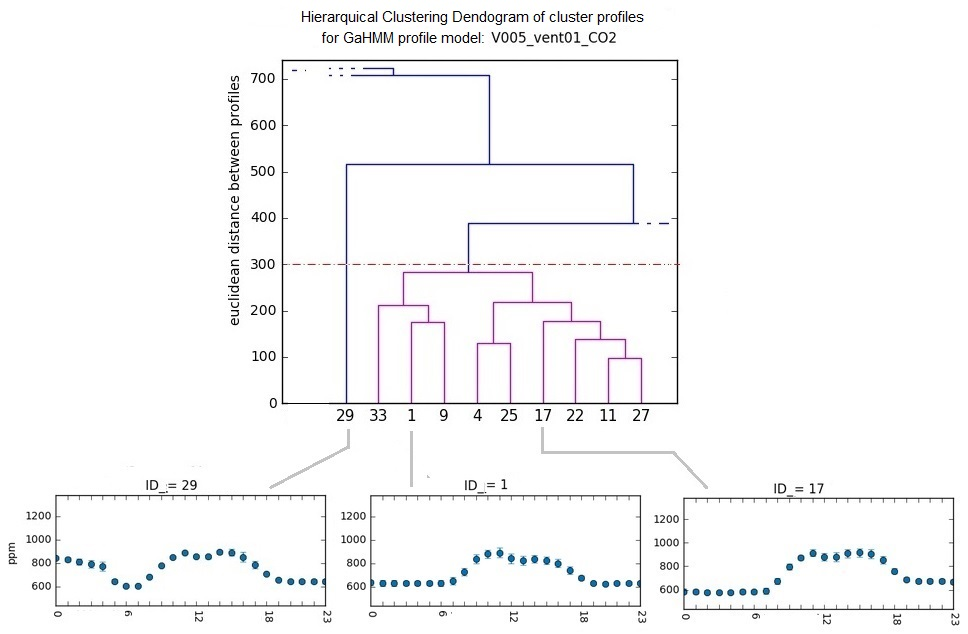
\includegraphics[scale=0.65]{Figures/dendrogram_CO2_NE.jpg}
  \caption{ Extract of the resulting hierarchical clustering dendrogram for the observed matrix $M$ using the $CO_2$ cluster profiles of the North-East ventilation system.}
  \label{fig:dendrogram_CO2_NE}
\end{figure} 

\textit{Step d)} The resulting dendrogram of the hierarchical clustering can be obtained by using the dendrogram's plot method of the clustering package of SciPy \footnote{Dendrogram method available on: \url{https://docs.scipy.org/doc/scipy-0.14.0/reference/generated/scipy.cluster.hierarchy.dendrogram.html}}. Figure \ref{fig:dendrogram_CO2_NE} shows an extract of the resulting dendrogram for the $CO_2$ cluster profiles for the North-East ventilation system. We observe that the cluster profiles $ID_x = [33, 1, 9, 4, 25, 17, 22, 11, 27]$ are very similar to each other (Figure \ref{fig:CO2_candidates_comparison}), however this is not the case for the cluster profile $ID_y=29$. This fact is remarkable when we observe the similarity metric (i.e. euclidean distance using the average linkage method) between cluster $ID_y=29$ and any profile of $ID_x$. Based on this similarity metric, we can conclude that clusters of $ID_x$ do not match with $ID_y$ and therefore they are two different classes of patterns. Looking at the differences in profile $ID_y = 29$, we observe an abnormal fluctuation, that is, that the $CO_2$ levels are above $800 \ ppm$ at the very beginning of the day  which is contrary to the normal level $\approx [400 - 650] \ ppm$. Thus, we can conclude that clusters of $ID_x$ should be part of the motif clusters and clusters of $ID_y$ should be part of the discord clusters. 

\begin{figure}[h!]
  \vspace{0.5em} %better style
  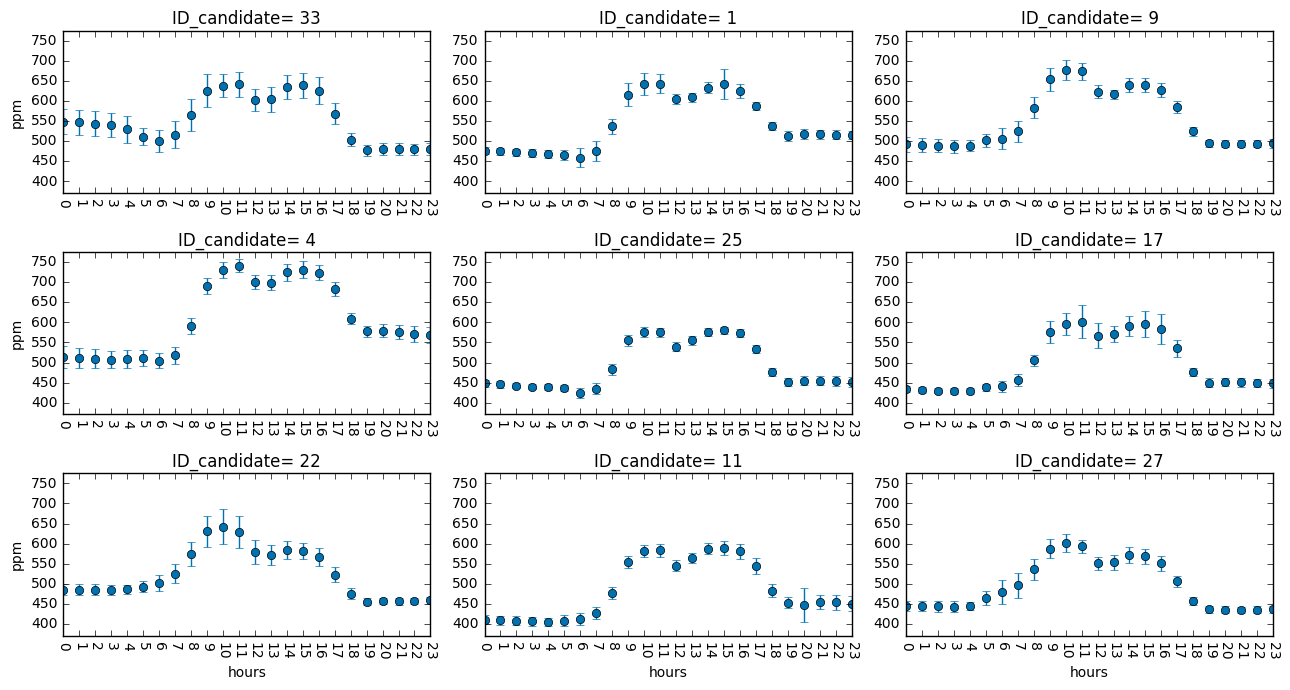
\includegraphics[scale=0.5]{Figures/CO2_candidates_comparison.jpg}
  \caption{$CO_2$ cluster profiles \textit{$ID_x$ = [33, 1, 9, 4, 25, 17, 22, 11, 27]} for the North-East ventilation system.}
  \label{fig:CO2_candidates_comparison}
\end{figure}  

Heuristically, we define an euclidean distance of 300 as a cut-off limit in the resulting dendrograms for the two systems (\ref{fig:dendrogram_CO2_NE_complete}, \ref{fig:dendrogram_CO2_SW_complete}), this allows to discriminate the discord and motif profiles. The cut-off value creates 11 hierarchical clusters (\ref{tab:h_cluster_all}) in the hierarchical clustering dendrogram of the North-East ventilation system (annex \ref{fig:dendrogram_CO2_NE_complete}). One can observe that the clusters are joined together in a hierarchical fashion from the closest, that is most similar (i.e. shorter distance), to the furthest apart, that is the most different (i.e. larger distance). Those clusters that join other clusters at further distances over 300 are considered as discord clusters because they differ more than the average of clusters. These discord cluster profiles (i.e. \textit{[30, 3, 13, 18, 20, 10, 31, 29}) can be appreciated in annex \ref{fig:discord_candidates_all}. The same cut-off value was applied for the hierarchical clustering dendrogram of the $CO_2$ clusters of the South-West ventilation system (annex \ref{fig:dendrogram_CO2_SW_complete}). We found in this case 4 hierarchical clusters (\textit{[B1, B2, B3, B4]}) as is shown in table \ref{tab:h_cluster_all}. However, there is no clusters that join other clusters at distances greater than 300. Looking at all the clusters for the South-West system (\ref{fig:candidates_profiles_SW}) we observe that all of them follow an "uniform" pattern and there is no big difference at first glance. Nevertheless, we decided to spot those cluster profiles that diverge slightly from the rest of the clusters in the South-West ventilation system, so for that we created a new cut-off value of 200 and found clusters \textbf{ID=23, 28, 34} (see annex \ref{fig:discord_candidates_all_SW}). These clusters represent mostly high $CO_2$ levels on the winter period but this fluctuation is still close to the normal. One can observe therefore that a threshold between 200 and 300 is a good value for detecting abnormal fluctuations for both ventilation systems.  \\

% Table generated by Excel2LaTeX from sheet 'hierarchical clustering'
\begin{table}[htbp]
  \centering
  \scriptsize
  \caption{Hierarchical clustering for a) $CO_2$ clusters of the North-East ventilation system b) $CO_2$ clusters of the South-West ventilation system}
       \begin{tabular}{|l|l|l|rrr}
    \multicolumn{3}{c}{a) North-East ventilation system} &      & \multicolumn{2}{c}{b) South-West ventilation system} \bigstrut[b]\\
\cline{1-3}\cline{5-6}    \rowcolor[rgb]{ .851,  .851,  .851} \textbf{Observation} & \textbf{Hierarchical} & \multicolumn{1}{c|}{\textbf{V005\_vent01\_CO2 (CO2 levels)}} & \multicolumn{1}{r|}{\cellcolor[rgb]{ 1,  1,  1} } & \multicolumn{1}{l|}{\textbf{Hierarchical}} & \multicolumn{1}{c|}{\textbf{V022\_vent02\_CO2 (CO2 levels)}} \bigstrut[t]\\
    \rowcolor[rgb]{ .851,  .851,  .851}      & \textbf{Cluster ID} & \multicolumn{1}{c|}{\textbf{cluster ID}} & \multicolumn{1}{r|}{\cellcolor[rgb]{ 1,  1,  1} } & \multicolumn{1}{l|}{\textbf{cluster ID}} & \multicolumn{1}{c|}{\textbf{Cluster ID}} \bigstrut[b]\\
\cline{1-3}\cline{5-6}    motif & \cellcolor[rgb]{ .949,  .949,  .949} \textbf{A1 } & [2, 7, 21, 28]  & \multicolumn{1}{r|}{} & \multicolumn{1}{l|}{\cellcolor[rgb]{ .949,  .949,  .949} \textbf{B1}} & \multicolumn{1}{l|}{[4, 13, 28]} \bigstrut\\
\cline{1-3}\cline{5-6}    motif & \cellcolor[rgb]{ .949,  .949,  .949} \textbf{A2} & [6, 19, 26]  & \multicolumn{1}{r|}{} & \multicolumn{1}{l|}{\cellcolor[rgb]{ .949,  .949,  .949} \textbf{B2}} & \multicolumn{1}{l|}{[2, 6, 8, 14, 18, 21, 23, 24, 29, 31]} \bigstrut\\
\cline{1-3}\cline{5-6}    motif & \cellcolor[rgb]{ .949,  .949,  .949} \textbf{A3} & [0, 5, 8, 12, 14, 15, 16, 23, 24, 32]  & \multicolumn{1}{r|}{} & \multicolumn{1}{l|}{\cellcolor[rgb]{ .949,  .949,  .949} \textbf{B3}} & \multicolumn{1}{l|}{[0, 3, 10, 11, 17, 20, 25, 27, 34]} \bigstrut\\
\cline{1-3}\cline{5-6}    motif & \cellcolor[rgb]{ .949,  .949,  .949} \textbf{A4} & [1, 4, 9, 11, 17, 22, 25, 27, 33]  & \multicolumn{1}{r|}{} & \multicolumn{1}{l|}{\cellcolor[rgb]{ .949,  .949,  .949} \textbf{B4}} & \multicolumn{1}{l|}{[1, 5, 7, 9, 12, 15, 16, 19, 22, 26, 30, 32, 33]} \bigstrut\\
\cline{1-3}\cline{5-6}    discord & \cellcolor[rgb]{ .949,  .949,  .949} \textbf{A5} & [30]  &      &      &  \bigstrut\\
\cline{1-3}    discord & \cellcolor[rgb]{ .949,  .949,  .949} \textbf{A6} & [3]  &      &      &  \bigstrut\\
\cline{1-3}    discord & \cellcolor[rgb]{ .949,  .949,  .949} \textbf{A7} & [13]  &      &      &  \bigstrut\\
\cline{1-3}    discord & \cellcolor[rgb]{ .949,  .949,  .949} \textbf{A8} & [18]  &      &      &  \bigstrut\\
\cline{1-3}    discord & \cellcolor[rgb]{ .949,  .949,  .949} \textbf{A9} & [20]  &      &      &  \bigstrut\\
\cline{1-3}    discord & \cellcolor[rgb]{ .949,  .949,  .949} \textbf{A10} & [10, 31]  &      &      &  \bigstrut\\
\cline{1-3}    discord & \cellcolor[rgb]{ .949,  .949,  .949} \textbf{A11} & [29]  &      &      &  \bigstrut\\
\cline{1-3}    \end{tabular}%
  \label{tab:h_cluster_all}%
\end{table}%


We showed in this way, how our proposed approach \textit{GaHMM-profile model} in combination with the hierarchical agglomerative clustering allow us to identify potential discord clusters and motif clusters. \\


\subparagraph{\textit{Interpretation of the results}} 

As we can see on the resulting dendrograms [\ref{fig:dendrogram_CO2_NE_complete}, \ref{fig:dendrogram_CO2_SW_complete}] and the hierarchical agglomerative clustering table {\ref{tab:h_cluster_all}}, the tree dendrogram structure for the $CO_2$ clusters of the North-East ventilation system is not as homogeneous as the South-West ventilation system. This is because in the North-East ventilation system, there are some particular cluster profiles that behave very differently from the majority of the clusters. These particular clusters join the tree schema at a very latter level, and therefore, can be classified as discord profiles. We conclude that the North-East ventilation system suffered some kind of anomaly, because cluster profiles $ID=3; 13; 18; 20; 29; 30$ do not appear frequently and they show clearly a weird behavior that is not appropriated, and furthermore, they are not present on the South-West ventilation system. For example the cluster 18 starts the day with 800 ppm which is approximately 250 ppm more than the usual value ($\approx [450 - 650]$ ppm), this $CO_2$ level and the additional accumulation of $CO_2$ coming from the occupants provoked an excessive $CO_2$ level of over 1300 ppm in the afternoon. Another example is the cluster 13 that presents low levels at the beginning of the day, and then, the levels increase in an unexpected way, finishing the day with the highest levels of $CO_2$ very close to the threshold of $1000 \ ppm$. These kind of situations are not present on the South-West ventilation system where the maximum $CO_2$ level is not higher than 870 ppm. To verify this fact, is enough to check the daily profiles that belong to the clusters $ID = 28; 4; 13$ of the South-West ventilation system (annex \ref{fig:discord_candidates_all_SW}) since they have the highest $CO_2$ levels. Finally, the GaHMM-profile model allows us to spot 61 atypical days for the North-East ventilation system and 17 atypical days for the South-West ventilation system of a total of 1081 days. More details about the detected anomalies for the North-East system are exposed in the case study, in section \ref{section:case_study_1}  \\  


\subsection{Case study:  North-East ventilation system}

\label{section:case_study_1}

As pointed out in section \ref{section:CO2_analysis} the North East ventilation system presents some $CO_2$ anomalous profiles that were clustered as discord profiles (annex \ref{fig:discord_candidates_all}). In this section, we analyze in details these profiles and we show their linkage with other associated variables. To show this linkage, in a similar fashion to how we spotted motif and discord clusters for the $CO_2$ measurements, we use the individual \textit{GaHMM - profile} models and their correspondent hierarchical agglomerative clustering, for spotting discord cluster profiles. The variables used to do this analysis are: \textit{exhaust air temperature, intake air temperature, humidity of the exhausted air of the ventilation system, heating TABS comsuption (KWh) and temperature in rooms}. Each variable has his
own \textit{GaHMM profile model} and the respective hierarchical agglomerative dendrograms. The complete list of cluster profiles of each variable are included as a digital annex in directory: \textit{/Thesis\_project/iPythonBooks/Diversity of profiles}, and additionally, the hierarchical agglomerative dendrograms for each variable is in annexes \ref{fig:dendrogram_exhausted_NE}, \ref{fig:dendrogram_intake_NE}, \ref{fig:dendrogram_exhausted_humidity_NE}, \ref{fig:dendrogram_room_temperature_NE} and \ref{fig:dendrogram_heating_NE}. 


We use all our proposed models (i.e. \textit{GaHMM seasonal, interactional and profile models}) to construct a data frame with all the labels produced by each model. Table \ref{tab:data_frame} shows an example of how this data frame looks like\footnote{Labels \textit{t\_period\_1} and \textit{t\_period\_2} refers the \textit{hottest transition} and \textit{coldest transition} respectively.}. All of this information helps to spot atypical/typical cluster profiles across seasons, interactional regimen and years. One can use different filters according to the research interests. For example, one obtains the figure \ref{fig:winter_vs_summer} by using the filter "\textit{winter, regime NC and working days}". This bar plot describes the distribution of cluster profiles using the $ID_{profile}$ of three of the analyzed variables. In the first case, the $CO_2$ cluster profile $ID=32$ is the typical profile for working days in winter period, while the cluster profile $ID=8$ is the typical profile for summer period. Note that cluster profiles that exist in winter period do not necessarily appear in summer.     

% Table generated by Excel2LaTeX from sheet 'Hoja3'
\begin{table}[htbp]
  \centering
  \tiny
  \caption{DataFrame includes labels of interactional, seasonal and profile \textit{GaHMM models}. Each profile model is named using the name of the correspondent variable.}
    \begin{tabular}{|c|r|r|r|r|r|r|r|r|r|}
\cline{6-10}    \multicolumn{1}{r}{} & \multicolumn{1}{r}{} & \multicolumn{1}{r}{} & \multicolumn{1}{r}{} &      & \multicolumn{5}{c|}{GaHMM profile models (ID\_profile)} \bigstrut\\
    \hline
    \rowcolor[rgb]{ 1,  .753,  0} \multicolumn{1}{|l|}{\textbf{timestamp }} & \multicolumn{1}{l|}{\textbf{weekday}} & \multicolumn{1}{l|}{\textbf{day\_type }} & \multicolumn{1}{l|}{\textbf{interaction}} & \multicolumn{1}{l|}{\textbf{season }} & \multicolumn{1}{l|}{\textbf{V005\_}} & \multicolumn{1}{l|}{\textbf{V006\_vent01}} & \multicolumn{1}{l|}{\textbf{V012\_vent01}} & \multicolumn{1}{l|}{\textbf{V004\_vent01}} &  \bigstrut[t]\\
    \rowcolor[rgb]{ 1,  .753,  0}      &      &      & \multicolumn{1}{l|}{\textbf{label}} & \multicolumn{1}{l|}{\textbf{label}} & \multicolumn{1}{l|}{\textbf{vent01\_CO2 }} & \multicolumn{1}{l|}{\textbf{\_temp\_out }} & \multicolumn{1}{l|}{\textbf{\_temp\_in }} & \multicolumn{1}{l|}{\textbf{\_hum\_out }} & \multicolumn{1}{l|}{\textbf{…}} \bigstrut[b]\\
    \hline
    \multicolumn{1}{|r|}{23-Jun-12} & \multicolumn{1}{l|}{Saturday } & \multicolumn{1}{l|}{weekend } & \multicolumn{1}{l|}{Reg. PC } & \multicolumn{1}{l|}{summer } & 21   & 35   & 2    & 0    & \multicolumn{1}{l|}{\textbf{…}} \bigstrut\\
    \hline
    \multicolumn{1}{|r|}{24-Jun-12} & \multicolumn{1}{l|}{Sunday } & \multicolumn{1}{l|}{weekend } & \multicolumn{1}{l|}{Reg. WC } & \multicolumn{1}{l|}{summer } & 21   & 1    & 2    & 12   &  \bigstrut\\
    \hline
    \multicolumn{1}{|r|}{25-Jun-12} & \multicolumn{1}{l|}{Monday } & \multicolumn{1}{l|}{working\_day } & \multicolumn{1}{l|}{Reg. NC } & \multicolumn{1}{l|}{summer } & 8    & 11   & 3    & 33   &  \bigstrut\\
    \hline
    \multicolumn{1}{|r|}{26-Jun-12} & \multicolumn{1}{l|}{Tuesday } & \multicolumn{1}{l|}{working\_day } & \multicolumn{1}{l|}{Reg. NC } & \multicolumn{1}{l|}{summer } & 8    & 7    & 3    & 33   &  \bigstrut\\
    \hline
    …    &      &      &      &      &      &      &      &      &  \bigstrut\\
    \hline
    \end{tabular}%
  \label{tab:data_frame}%
\end{table}%


\begin{figure}[h!]
  \vspace{0.5em} %better style
  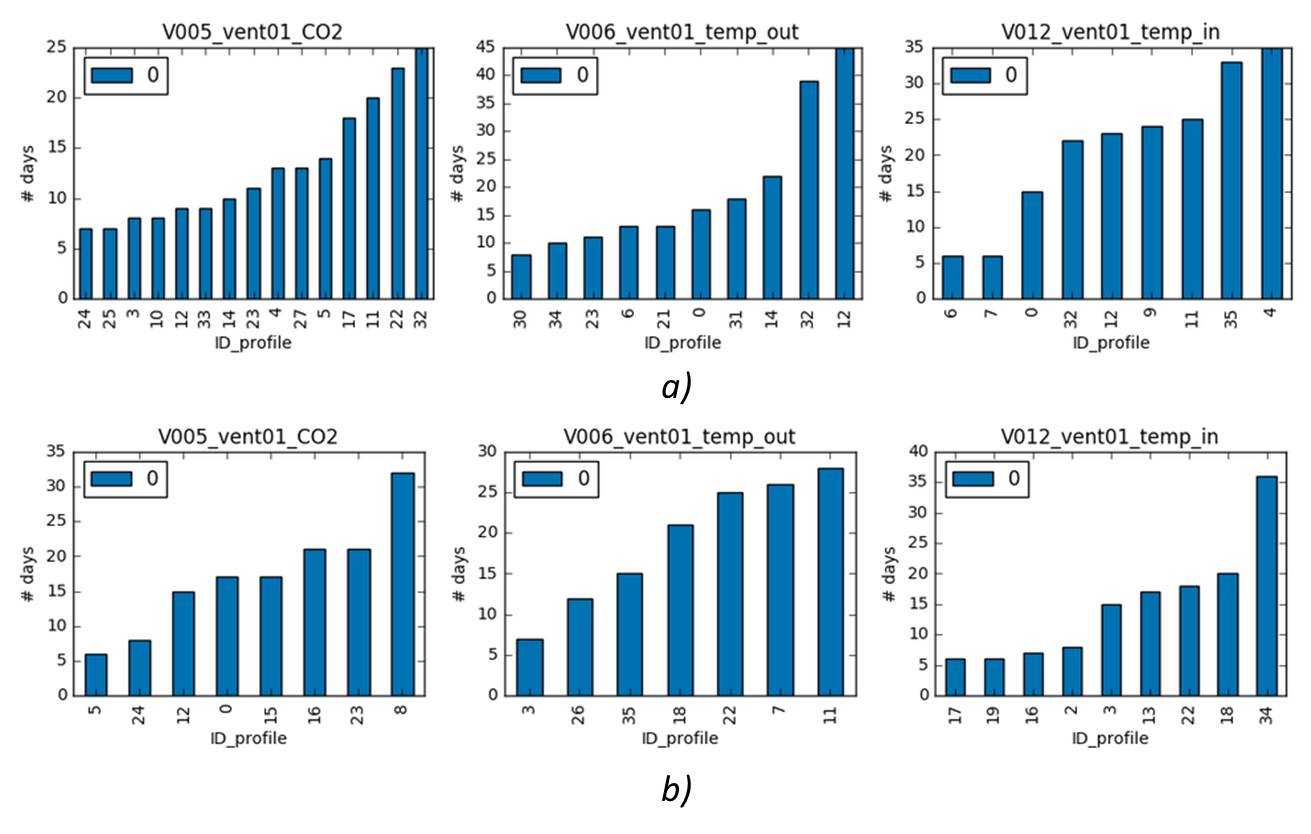
\includegraphics[scale=0.7]{Figures/cluster_dist_winter_summer.jpg}
  \caption{Distribution of cluster profiles (i.e. $ID_{profile}$) for working days: \textit{a)} winter period, b) summer period.}
  \label{fig:winter_vs_summer}
\end{figure} 

We use dendrograms: \ref{fig:dendrogram_exhausted_NE}, \ref{fig:dendrogram_intake_NE}, \ref{fig:dendrogram_exhausted_humidity_NE}, \ref{fig:dendrogram_room_temperature_NE} and \ref{fig:dendrogram_heating_NE} to spot the discord cluster profiles (i.e. the thick blue lines). At the end of the filter process, we discover a temporal coincidence of the discord profiles between variables. This is shown in a calendar visualization in figure \ref{fig:case-study}. 

Each small square represents a discord profile that was found by performing the process in section \ref{sec:discord_finding}. One can see a pattern of discord profiles, that is the set of blue violet and green squares, corresponding to the variables: \textit{$CO_2$ levels, exhaust air temperature and intake air temperature of the ventilation system}. This pattern is a group of discords of different variables that appears all together. In contrast, variables: \textit{humidity of the exhausted air, heating TABS comsuption (KWh) and temperature in rooms} have an occasional temporal coincidence, but this is not so evident as the later case. At least 15 atypical weeks were spotted using this approach. To exemplify one of them, we show the case that appears in period \textit{December 03 to December 13, 2012}. Figure \ref{fig:normal_period} shows the normal trend of the $CO_2$ levels for the ventilation system two week before the fault,and the next figure \ref{fig:fault_period} shows the moment when the fault occurs. One can see that the $CO_2$ levels are excessive, reaching levels greater than 1000 ppm. In the bottom part, we include the sequence of ID discord clusters. It is identifiable that the fault sequence starts with clusters \textit{13, 3} and finishes with clusters \textit{18, 10, 26}. We observe that the same phenomena occurs with some variations on November 2012, February 2013, December 2013, and with lesser impact on 2014 and 2015. The annex \ref{fig:sequence_candidates} shows the sequence of discord clusters where one can appreciate the different patterns that occur during the faults. 
    
\begin{figure}[h!]
  \vspace{0.5em} %better style
  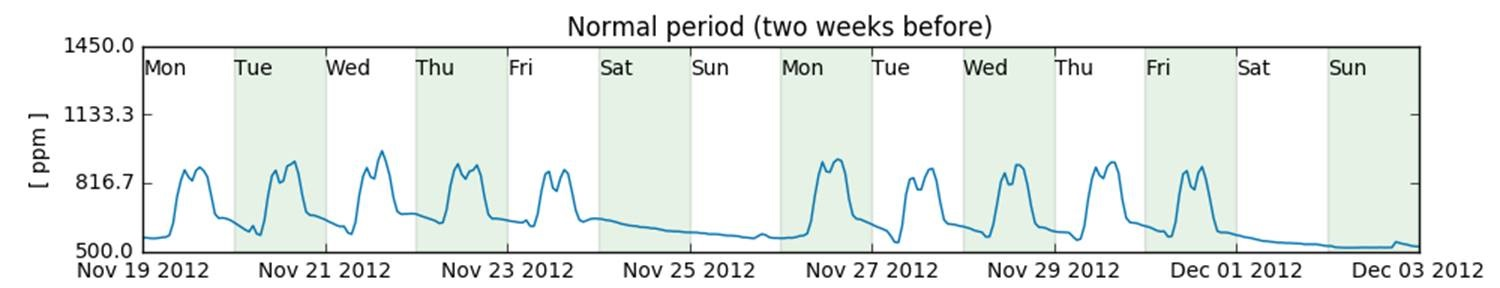
\includegraphics[scale=0.6]{Figures/case_study_trend_1_normal.jpg}
  \caption{Levels of $CO_2$ of the ventilation system during a normal period.}
  \label{fig:normal_period}
\end{figure}

\begin{figure}[h!]
  \vspace{0.5em} %better style
  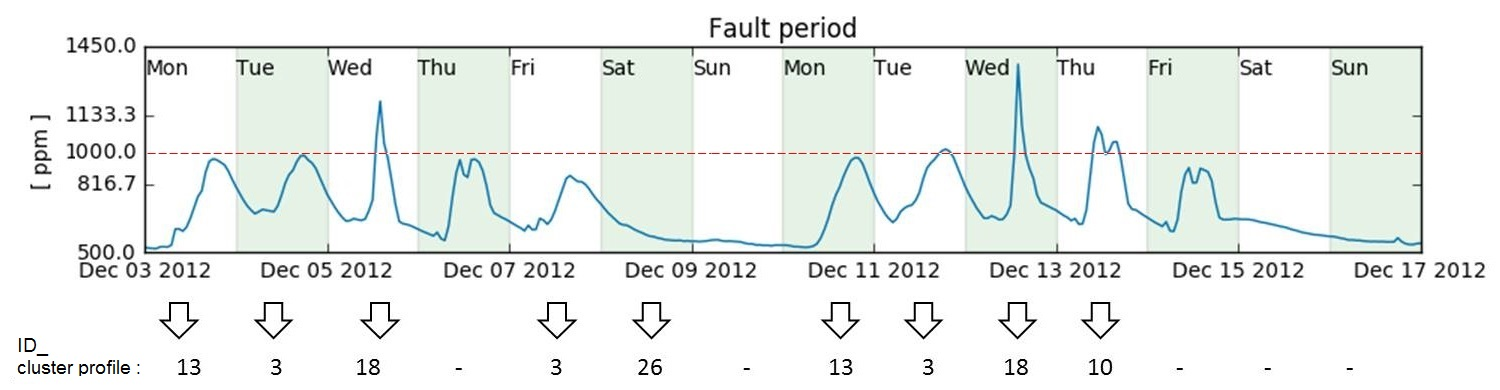
\includegraphics[scale=0.6]{Figures/case_study_trend_1_fault.jpg}
  \caption{$CO_2$ levels in the North-East ventilation system during the fault period. In the bottom part, the ID of the discord clusters shows the sequence of the fault.}
  \label{fig:fault_period}
\end{figure}

Figure \ref{fig:complete_fault_trends} shows on the left hand side, the normal trend of the analyzed variables, and on the right hand side, the trend of the variables in the fault period. The red line under each variable trend indicates that these daily profiles were spotted as discord cluster profiles. One can observe the temporal coincidence of discord profiles. Table \ref{tab:fault_dataframe} presents an example of the label data frame with information from all the models before and during the fault period. The red number in bold implies discord cluster profiles.


\begin{figure}[h!]
  \vspace{0.5em} %better style
  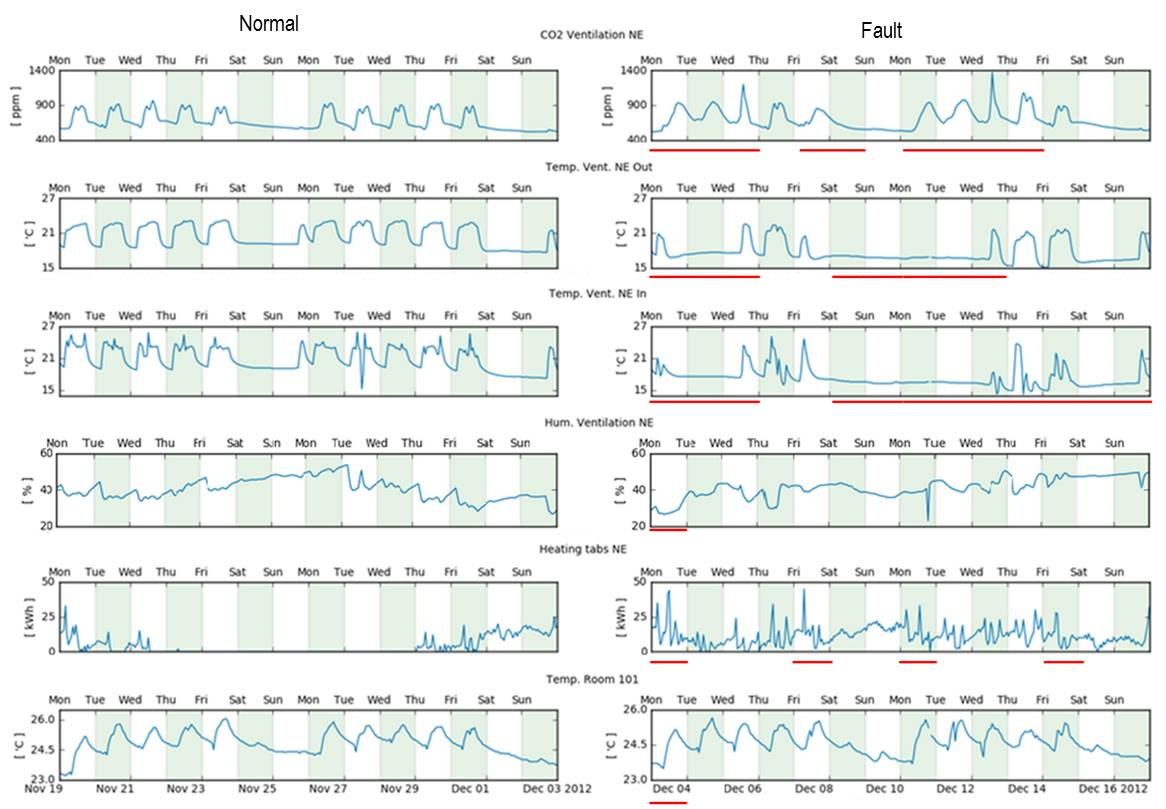
\includegraphics[scale=0.82]{Figures/complete_fault_trends.jpg}
  \caption{Trend of analyzed variables in period: December 03 to December 13, 2012.}
  \label{fig:complete_fault_trends}
\end{figure}


% Table generated by Excel2LaTeX from sheet 'Hoja4'
\begin{table}[htbp]
  \centering
  \tiny
  \caption{Label data frame with information from all the GaHMM models.}
    \begin{tabular}{|c|c|c|c|c|c|c|c|c|}
    \hline
    \textit{\textbf{timestamp}} & \textit{\textbf{Regime}} & \textit{\textbf{Season}} & \textit{\textbf{CO2\_}} & \textit{\textbf{Exhaust air}} & \textit{\textbf{Intake air}} & \textit{\textbf{Exhaust air}} & \textit{\textbf{Heating}} & \textit{\textbf{Room 101}} \bigstrut[t]\\
         &      &      & \textit{\textbf{Ventilation}} & \textit{\textbf{Temperature}} & \textit{\textbf{Temperature}} & \textit{\textbf{Humidity}} & \textit{\textbf{TABS (kWh)}} & \textit{\textbf{Temperature}} \bigstrut[b]\\
    \hline
    Mon, Nov 26, 2012 & NC   & t\_period\_2 & 17   & 24   & 12   & 23   & 1    & 30 \bigstrut\\
    \hline
    Tue, Nov 27, 2012 & NC   & winter & 22   & 30   & 12   & 19   & 1    & 0 \bigstrut\\
    \hline
    Wed, Nov 28, 2012 & NC   & winter & 22   & 6    & 12   & 30   & 1    & 7 \bigstrut\\
    \hline
    Thu, Nov 29, 2012 & WC   & winter & 22   & 31   & 12   & 15   & 5    & 13 \bigstrut\\
    \hline
    Fri, Nov 30, 2012 & WC   & winter & 5    & 31   & 0    & 34   & 12   & 13 \bigstrut\\
    \hline
    Sat, Dec 01, 2012 & PC   & winter & 28   & 5    & 24   & 15   & 0    & 3 \bigstrut\\
    \hline
    Sun, Dec 02, 2012 & NC   & winter & 21   & 20   & 5    & 34   & 16   & 9 \bigstrut\\
    \hline
    \rowcolor[rgb]{ .988,  .835,  .706} Mon, Dec 03, 2012 & \textbf{WC} & winter & \textcolor[rgb]{ 1,  0,  0}{\textbf{13}} & \textcolor[rgb]{ 1,  0,  0}{\textbf{27}} & \textcolor[rgb]{ 1,  0,  0}{\textbf{1}} & \textcolor[rgb]{ 1,  0,  0}{\textbf{5}} & \textcolor[rgb]{ 1,  0,  0}{\textbf{21}} & \textcolor[rgb]{ 1,  0,  0}{\textbf{29}} \bigstrut\\
    \hline
    \rowcolor[rgb]{ .988,  .835,  .706} Tue, Dec 04, 2012 & \textbf{WC} & winter & \textcolor[rgb]{ 1,  0,  0}{\textbf{3}} & \textcolor[rgb]{ 1,  0,  0}{\textbf{5}} & \textcolor[rgb]{ 1,  0,  0}{\textbf{24}} & \cellcolor[rgb]{ 1,  1,  1} 15 & \cellcolor[rgb]{ 1,  1,  1} 5 & \cellcolor[rgb]{ 1,  1,  1} 32 \bigstrut\\
    \hline
    \rowcolor[rgb]{ .988,  .835,  .706} Wed, Dec 05, 2012 & \textbf{WC} & winter & \textcolor[rgb]{ 1,  0,  0}{\textbf{18}} & \textcolor[rgb]{ 1,  0,  0}{\textbf{17}} & \textcolor[rgb]{ 1,  0,  0}{26} & \cellcolor[rgb]{ 1,  1,  1} 15 & \cellcolor[rgb]{ 1,  1,  1} 19 & \cellcolor[rgb]{ 1,  1,  1} 13 \bigstrut\\
    \hline
    \rowcolor[rgb]{ .988,  .835,  .706} Thu, Dec 06, 2012 & \textbf{WC} & winter & \cellcolor[rgb]{ 1,  1,  1} 17 & \cellcolor[rgb]{ 1,  1,  1} 0 & \cellcolor[rgb]{ 1,  1,  1} 27 & \cellcolor[rgb]{ 1,  1,  1} 15 & \cellcolor[rgb]{ 1,  1,  1} 24 & \cellcolor[rgb]{ 1,  1,  1} 32 \bigstrut\\
    \hline
    \rowcolor[rgb]{ .988,  .835,  .706} Fri, Dec 07, 2012 & \textbf{WC} & winter & \textcolor[rgb]{ 1,  0,  0}{\textbf{3}} & \textcolor[rgb]{ 1,  0,  0}{\textbf{27}} & \cellcolor[rgb]{ 1,  1,  1} 27 & \cellcolor[rgb]{ 1,  1,  1} 30 & \textcolor[rgb]{ 1,  0,  0}{\textbf{8}} & \cellcolor[rgb]{ 1,  1,  1} 32 \bigstrut\\
    \hline
    \rowcolor[rgb]{ .988,  .835,  .706} Sat, Dec 08, 2012 & \textbf{WC} & winter & \textcolor[rgb]{ 1,  0,  0}{\textbf{26}} & \textcolor[rgb]{ 1,  0,  0}{\textbf{5}} & \textcolor[rgb]{ 1,  0,  0}{\textbf{24}} & \cellcolor[rgb]{ 1,  1,  1} 30 & \cellcolor[rgb]{ 1,  1,  1} 18 & \cellcolor[rgb]{ 1,  1,  1} 3 \bigstrut\\
    \hline
    Sun, Dec 09, 2012 & WC   & winter & 28   & \cellcolor[rgb]{ .988,  .835,  .706} \textcolor[rgb]{ 1,  0,  0}{\textbf{5}} & \cellcolor[rgb]{ .988,  .835,  .706} \textcolor[rgb]{ 1,  0,  0}{\textbf{6}} & 15   & 14   & 23 \bigstrut\\
    \hline
    \end{tabular}%
  \label{tab:fault_dataframe}%
\end{table}%

Finally, we observe that the fault detailed in figure \ref{fig:complete_fault_trends} disappears after the discovered maintenance period (section \ref{sec:interactional_results}). 
We probed this by doing the filtering process in the label data frame (i.e. \ref{tab:data_frame}) that the daily profiles had changed after the discovered maintenance period. We probe the last fact by performing the \textit{Welch's t-test} \footnote{We use the package \url{https://docs.scipy.org/doc/scipy-0.19.0/reference/generated/scipy.stats.ttest_ind.html}, the digital annex file is: \textit{iPythonBooks/t-test}} over different days, giving rise to the following results:

\begin{itemize}
\item There was a significant difference in the scores for the $CO_2$ levels before the maintenance period (M=568 ppm, SD=18.24) and after the maintenance period (M=451 ppm, SD=21.25) for Saturdays; t(956)= -30.85, p=0.00001.  
\item There was a significant difference in the scores for the $CO_2$ levels before the maintenance period (M=698.9 ppm, SD=81.47) and after the maintenance period (M=672.2 ppm, SD=21.71) for the typical cluster profiles of working days; t(1500)= 5.91, p=0.00001. The typical profiles before the maintenance period are cluster profiles $ID=[32; 22]$ and after the maintenance, cluster profiles $ID=[12, 7]$.   
\end{itemize}

A jupyter notebook is included as a digital annex for this study case in \textit{iPythonBooks/case study}. It includes the rest of periods where the faults appeared, we observe a similar behavior in all the detected faults.   

\newgeometry{margin=1.5cm}
\begin{landscape}
\leavevmode
\newline

\begin{figure}[h!]
  \vspace{0.5em} %better style
  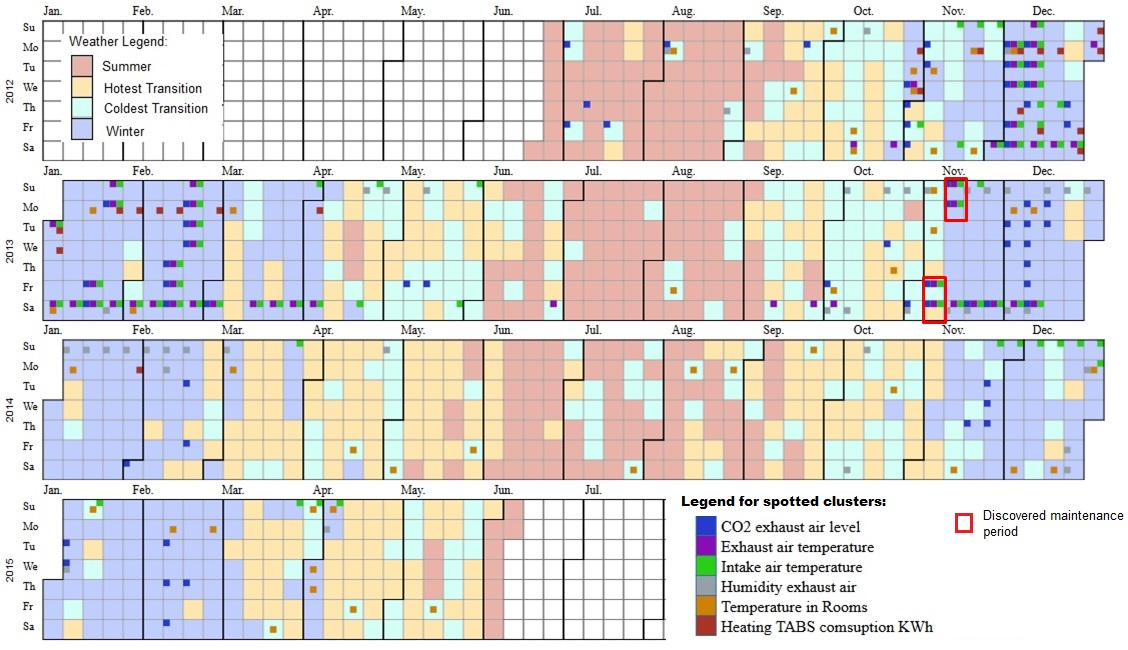
\includegraphics[scale=0.85]{Figures/case_study_complete.jpg}
  \caption{Case study: Discord cluster profiles of the North-East ventilation system.}
  \label{fig:case-study}
\end{figure}

\end{landscape}
\restoregeometry


\section{Practical application of the GaHMM-profile model}
\label{sec:pract_app}
\paragraph{Real time tracking} As it was demonstrate in last section, using our approach \textit{GaHMM-profile model} in combination with a hierarchical agglomerative clustering is an effective tool that assist stakeholders to define a threshold for detecting discord profiles in a system, and defining the motif profiles. 

The motif profiles are a good guide to knowing the typical fluctuations of a certain variable, and therefore one can use this information as a reference to spot potential abnormal fluctuations in real time \footnote{This is our proposition for a practical application of the \textit{GaHMM-profile} model. It requires further research, therefore is proposed as a future work in section \ref{future}}. To exemplify this practical application, we choose the $CO_2$ level time series and the correspondent motif clusters (see table \ref{tab:h_cluster_all}). We propose a simple routine that checks if the current trend is inside of an expected region \footnote{This script is implemented as: \textit{iPythonBooks/Application}}. This region can be defined by the collection of the motif cluster profiles where the current trend fits in. Figure \ref{fig:real_time_1} explains this concept, the red line is the current measurement of the $CO_2$ in an hourly fashion. One observes in these three trend graphs how the variable evolves along the day, and how the learned profiles (i.e. motif cluster profiles) provide the shape of the expected fluctuation for the variable (i.e. the green area). One also observe how little by little the area of the expected area becomes refined until the moment, where one or two cluster profile define the shape of the current measurement of the $CO_2$.  

\begin{figure}[h!]
  \vspace{0.5em} %better style
  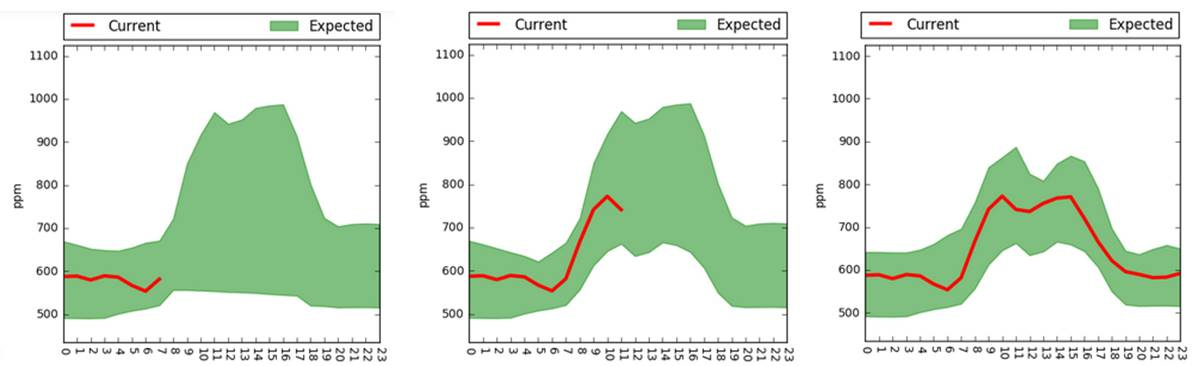
\includegraphics[scale=0.7]{Figures/real_time_1.jpg}
  \caption{Tracking the current $CO_2$ levels in the North-East ventilation system by using the correspondent motif cluster profiles of the \textit{GaHMM  profile model: V005\_vent01\_CO2}.}
  \label{fig:real_time_1}
\end{figure}

Figure \ref{fig:real_time_2} shows an example where an abnormal trend is detected because it does not fit inside of the motif cluster profiles. One observes how the routine tries to fit the expected area to the current trend, but at the end, one observes a divergence of 45\% (i.e. 13 values are inside of the green trend). These kinds of cases could be notified to the stakeholders for making decisions about these fluctuations, if for instance this problem is recurrent or there are suspicions that it is a serious problem.

\begin{figure}[h!]
  \vspace{0.5em} %better style
  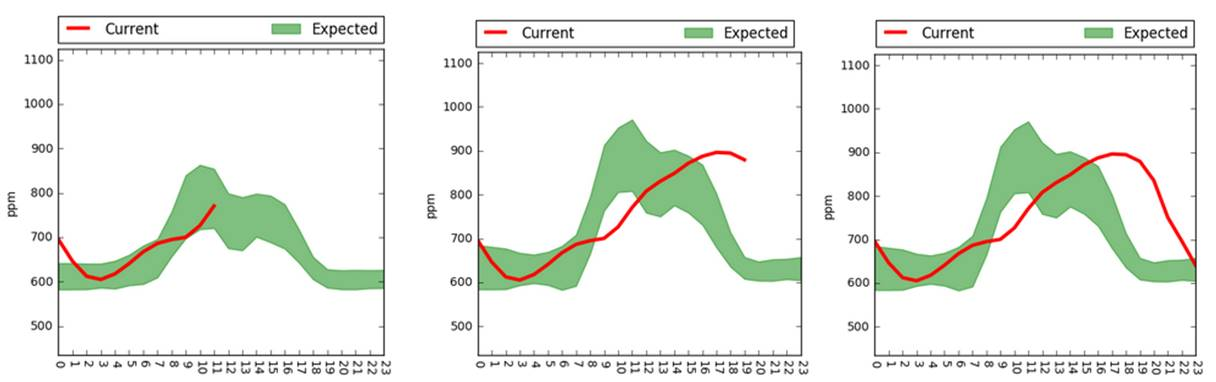
\includegraphics[scale=0.7]{Figures/real_time_2.jpg}
  \caption{Tracking the current $CO_2$ levels in the North-East ventilation system by using the correspondent motif cluster profiles of the \textit{GaHMM  profile model: V005\_vent01\_CO2}.}
  \label{fig:real_time_2}
\end{figure}

To know whether or not the current trend fits inside of a motif cluster profile, one uses the definition of a cluster profile, that is, the mean vector and the standard deviation vector. ($P_x = \{ \mu_{x_i} \forall i \in [0,23] \}$  and $STD_x = \{ \sigma_{x_i} \forall i \in [0,23] \}$). The upper and lower bound of a cluster profile are defined as: $U_{bound} = P_x + 1.5 \cdot STD_x$ and $L_{bound} = P_x - 1.5 \cdot STD_x$ \footnote{The constant 1.5 is arbitrary, nevertheless we use 1.5 because is the usual value used in Interquartile range analysis. Other values can be used as well.}. In this way, one routine checks if the current trend is inside of the intervals defined by the upper and lower bound. The collection $C$ of all the motif profiles where the current trend fits in defines the expected area. This expected area is defined as well by an upper and lower bound, that are the maximum and minimum values among all the cluster profile that belong to $C$. Therefore:


\begin{equation}
\begin{array}{lcl}
\textstyle  \text{Expected}_{area} & = & [$Lo$_{bound}, $Up$_{bound}] \\ \\
 $Lo$_{bound} & = & \displaystyle \min_{i=0,j=0}^{N,T} L_{bound} \in C  \\	\\
 $Up$_{bound} & = & \displaystyle \max_{i=0,j=0}^{N,T} U_{bound} \in C  	\\	\\
\end{array}
\end{equation}


Where $N$ is the total number of cluster profiles where the current trend fit in, and $T$ is the length of the current trend. We include a digital annex \textit{iPythonBooks/application} the routine that applies this practical application. We think that definition of the tracking time to use for knowing whether or not the current trend follows the typical pattern of fluctuation, should be defined by a specialist. We believe that this depends on the critical degree of a specific variable. It could be that one variable needs more control than others and therefore the recommend tracking time may need to be shorter. More further studies need to be done using our proposition, but at this time, this application remains as a future work.   
     

\section{Comparison between DayFilter approach and GaHMM approach}
\label{comparison_sax_hmm}
DayFilter approach is presented as a pattern recognition method that uses symbolic aggregate approximation (SAX), motif and discord extraction, and clustering to detect the underlying structure of building performance data \cite{kim2017review}. The original paper \cite{miller2015automated} uses building power measurement, but in our opinion, it can extended to any kind of measurements since it uses SAX as the core of the approach. SAX transformation is explained in section \ref{section:SAX} for further references. In this section, we explain the procedure that we performed to compare the result of DayFilter and GaHMM approach. Our intuition tell us if there is an anomalous sequence (i.e. discord cluster) that can be spotted by a corresponding SAX word, then we can spot all the sequences that match this word and compare these profiles with the \textit{GaHMM-profile model's} results. This is possible because the daily profile have same shape and similar magnitude for each point in the profile. Following this idea, we choose three variables that are directly associated with the occupants' comfort: ($CO_2$ level North-East zone, Temperature for room 101, Humidity for room 101). We applied the same process over the three variables. Only the time series of $CO_2$ level of the North East part of the building was chosen for illustration purposes in this section. Here the steps to follow:

\begin{itemize}
    	\item[a)] Select discord clusters that were found with \textit{GaHMM-profile model} for the variable of interest.
    	\item[b)] Using SAX transformation convert the selected discord cluster profiles in their corresponding SAX words.
    	\item[c)] Spot all the profiles that match with the corresponding SAX word, compare dates were both (GaHMM and SAX) have coincidence and tabulate the results.
    \end{itemize}
 
\begin{figure}[h!]
  \vspace{0.5em} %better style
  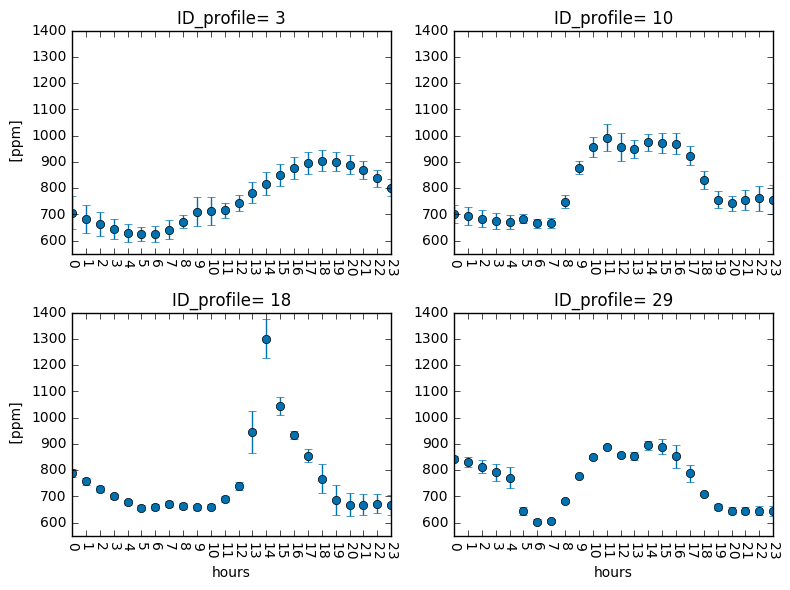
\includegraphics[scale=0.6]{Figures/discord_candidates_CO2.jpg}
  \caption{Example of $CO_2$ discord profiles for the North-East ventilation system. (4 of 11 profiles)}
  \label{fig:discord_candidates} 
\end{figure}
    
\textit{Step a)} After the training process of the \textit{GaHMM-profile model} for a specific variable (i.e. in this case $CO_2$ time series), we select the discord cluster profiles of interest\footnote{To know why these profiles were chosen as discord clusters, see section \ref{motif_results}}. The discord clusters profiles are defined by a mean vector $P_x = \{ \mu_{x_i} \forall i \in [0,23] \}$ and a standard deviation vector $STD_x = \{ \sigma_{x_i} \forall i \in [0,23] \}$ of length $N=24$, each value for each hour of the day. Figure \ref{fig:discord_candidates} shows examples of discord cluster profiles (\textit{profile identifier = [3,10,18,29]} ) and their corresponding values are included in annex \ref{tab:discord_profiles}. 

\textit{Step b)} The selected profiles are z-score normalized using the general mean $\mu_T$ and the general deviation standard $\sigma_T$. The values $\mu_T = 649.8 \ ppm$ and  $\sigma_T = 97.85 \ ppm$ were calculated using the entire time series where we remove the extreme points that fall outside of three standard deviations $x_i \not \in [\mu - 3\sigma, \mu + 3\sigma ]$. It should be noted that this must be calculated in this way to make it comparable to the DayFilter approach \cite{miller2015automated}. Additionally, we verify that the normalized data stream $Z(t)$ has an approximate 0 mean and a standard deviation of close to 1. The rest of the process of SAX transformation follows the procedure proposed by DayFilter \cite{lin2003symbolic, keogh2005hot, lin2007experiencing, miller2015automated}. We take the non-overlapping sub-sequence of length $N=24$ that was previously normalized, and we divided into W equal sized segments. Then the corresponding Piecewise Aggregate Approximation is performed \cite{lin2007experiencing}. Finally, each mean of the W segments are transformed in alphabetic characters by using the vertical breakpoints $B = \beta_1, ... \beta_{a-1}$ \cite{lin2007experiencing}. The definition of the breakpoint depends on the number of symbols to use for the SAX transformation (more information in section \ref{section:SAX}). \\

To make sure that the SAX transformation is correctly performed, we apply firstly this transformation over some motif clusters, this can be appreciated in Figure \ref{fig:motif_candidates_sax}. When we did this, we observed how the
letters were well distributed for each motif profile, therefore we conclude that the SAX transformation
is valid. Figure \ref{fig:discord_candidates_sax} shows the SAX transformation for each discord profile using parameters $W=4$,  $A=[a,b,c]$ and $B=[-0.43, 0.43]$. The corresponding SAX words for profiles 3, 10, 18, 29 are \textit{'bbcc', 'bccc', 'cbcb', 'cccb'}. \\

\begin{figure}[h!]
  \vspace{0.5em} %better style
  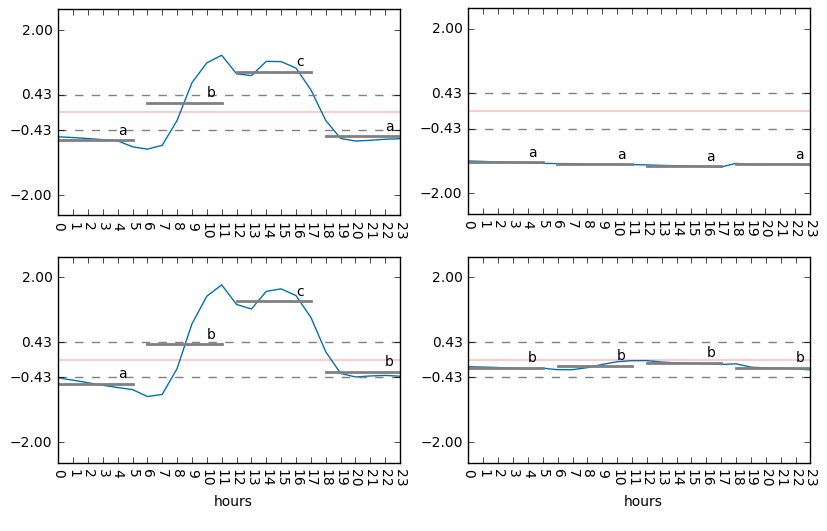
\includegraphics[scale=0.65]{Figures/motif_candidates_sax.jpg}
  \caption{Example of SAX transformation for \textbf{motif clusters} profiles. (4 of 23 profiles).}
  \label{fig:motif_candidates_sax}
\end{figure}

\begin{figure}[h!]
  \vspace{0.5em} %better style
  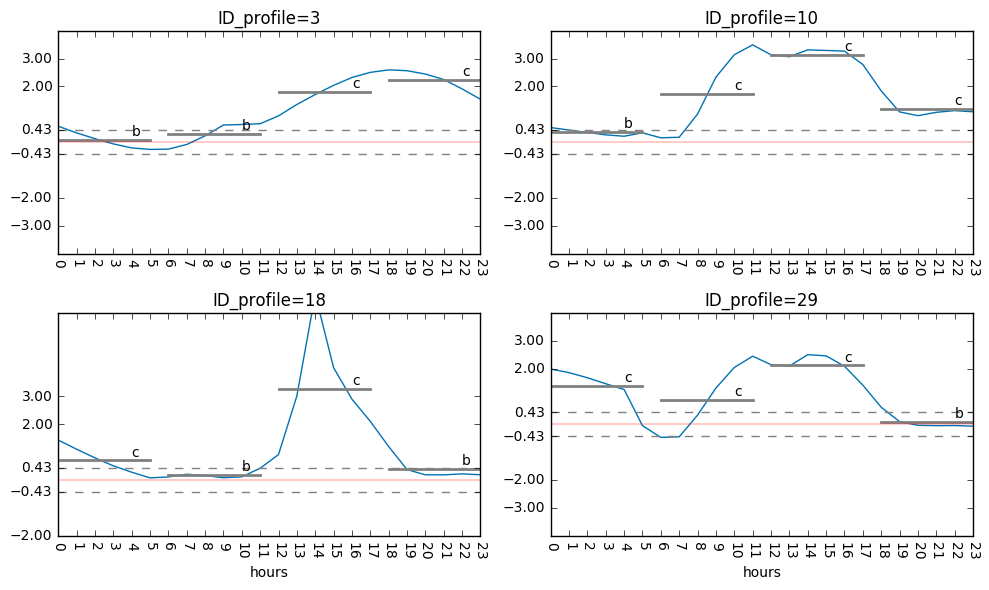
\includegraphics[scale=0.65]{Figures/discord_candidates_sax.jpg}
  \caption{Example of SAX transformation for \textbf{discord cluster profiles}. (4 of 11 profiles).}
  \label{fig:discord_candidates_sax}
\end{figure}


\textit{Step c)} To compare the dates where both approaches have coincidence, we perform SAX transformation over the entire time series changing the parameters $W$ and $A$. Then each daily profile is transformed in his respective word. We list the dates of profiles that match with each SAX word and then we compare against the dates that were found by GaHMM approach. Making $W >= 4$ and $|A| >=4 $ creates so much granularity that the comparison is not fair for SAX approach. In other words, a discord cluster profile ($P_x = \{ \mu_{x_i} \forall i \in [0,23] \}$  and $STD_x = \{ \sigma_{x_i} \forall i \in [0,23] \}$) can be broken down into so many combination of letters, so that the coincidence is lower. Having so much granularity makes difficult to define the set of words that belongs to this discord cluster. On the contrary, if we set $W<4$ and $|A|<4$ there is a risk to spot fake discord profiles that do not actually belong to the discord cluster, but were clustered by SAX due to the space between breakpoints. Table \ref{tab:SAX_vs_GaHMM} shows the results of this comparison.


% Table generated by Excel2LaTeX from sheet 'SAX vs GaHMM'
\begin{table}[htbp]
  \centering
  \scriptsize
  \caption{Number of days where the discord profiles were spotted by using \textit{GaHMM-profile model} and DayFilter approach. The corresponding coincidence of both approaches is done when both have the same date.}
    \begin{tabular}{|l|r|r|r|r|r|}
    \hline
         & \multicolumn{1}{l|}{\textbf{W = 4, |A|= 3}} & \multicolumn{1}{l|}{\textbf{W = 4, |A|= 4}} & \multicolumn{1}{l|}{\textbf{W = 4, |A|= 5}} & \multicolumn{1}{l|}{\textbf{W = 4, |A|= 6}} &  \bigstrut\\
    \hline
    \textbf{GaHMM} & 61   & 61   & 61   & 61   & days \bigstrut\\
    \hline
    \textbf{DayFilter} & 311  & 84   & 29   & 36   & days \bigstrut\\
    \hline
    \textbf{Coincidence} & 49   & 39   & 25   & 21   & days \bigstrut\\
    \hline
    \textbf{\% coincidence} & \cellcolor[rgb]{ .973,  .412,  .42} 15.2 & \cellcolor[rgb]{ .553,  .796,  .494} 36.8 & \cellcolor[rgb]{ .388,  .745,  .482} 38.5 & \cellcolor[rgb]{ .992,  .784,  .49} 27.6 & \% \bigstrut\\
    \hline
    \multicolumn{1}{r}{} & \multicolumn{1}{r}{} & \multicolumn{1}{r}{} & \multicolumn{1}{r}{} & \multicolumn{1}{r}{} & \multicolumn{1}{r}{} \bigstrut\\
    \hline
         & \multicolumn{1}{l|}{\textbf{W = 6, |A|= 3}} & \multicolumn{1}{l|}{\textbf{W = 6, |A|= 4}} & \multicolumn{1}{l|}{\textbf{W = 6, |A|= 5}} & \multicolumn{1}{l|}{\textbf{W = 6, |A|= 6}} &  \bigstrut\\
    \hline
    \textbf{GaHMM} & 61   & 61   & 61   & 61   & days \bigstrut\\
    \hline
    \textbf{DayFilter} & 49   & 33   & 19   & 16   & days \bigstrut\\
    \hline
    \textbf{Coincidence} & 29   & 25   & 17   & 15   & days \bigstrut\\
    \hline
    \textbf{\% coincidence} & \cellcolor[rgb]{ .443,  .761,  .486} 35.8 & \cellcolor[rgb]{ .388,  .745,  .482} 36.2 & \cellcolor[rgb]{ .98,  .608,  .455} 27.0 & \cellcolor[rgb]{ .973,  .412,  .42} 24.2 & \% \bigstrut\\
    \hline
    \end{tabular}%  
  \label{tab:SAX_vs_GaHMM}%
\end{table}%


We observe that both approaches have a maximum percentage of coincidence 
\footnote{When both approaches coincide on the same date, we define percentage of coincidence as: \\
$
	\% \ coincidence = \dfrac{\# \ coincidences}{\#\ GaHMM \ discords + \# \ FilterDay \ discords - \# \ coincidences} \cdot 100
$ } 
when $W=4, |A|= 5$. However, we consider more interesting the case when $W=4, |A|= 3$ because there is a maximum number of coinciding days, but DayFilter approach spots more discord profiles than \textit{GaHMM-profile model}. Looking deeper at the difference between both approaches we found that FilterDay approach spots some fakes profiles. Figure \ref{fig:fake_candidates} shows examples of fake profiles when we use SAX for spotting profiles corresponding to the word 'bccc' (profile 10) with $W=4, A=\{ a, b, c\}$. Observe how SAX is unable to define the changes that exists in profile 10 from 8h to 23h (i.e. Figure \ref{fig:discord_candidates_sax}) therefore the profile has a wide standard deviation and the $CO2$ level at hours 0-7 are lower than we expect for profile 10. We include more details about the dates when both approaches are coincident in annex \ref{viz:FilterDay_GaHMM}.  

\begin{figure}[h!]
  \vspace{0.5em} %better style
  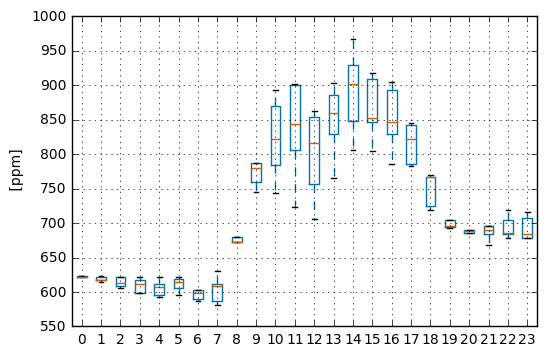
\includegraphics[scale=0.7]{Figures/fake_candidates.jpg}
  \caption{Example of fake profiles for cluster 10 ('bccc'), when FilterDay approach is applied with $W=4, |A|=3$.}
  \label{fig:fake_candidates}
\end{figure}

\subsubsection{Discussion about the experiment}

In this experiment, the over/underestimation of some discord profiles for the DayFilter approach is due to two aspects: the assumption that a z-score normalized time series has a Gaussian distribution  \cite{lin2003symbolic, keogh2005hot, lin2007experiencing, miller2015automated} and the wide space between the breakpoints. (\citeauthor{li2015encyclopedia}, \citeyear{li2015encyclopedia}) \cite{li2015encyclopedia} point out that a z-score normalization does not guarantee a Gaussian distribution, even if the mean of the normalized time series is aproximatly near to zero and the standard deviation close to one. Therefore, when SAX transformation is performed, some segments of the time series are not properly represented by the corresponding symbols. To overcome this problem, we could normalized each sample of size N as the original version of SAX suggests \cite{keogh2005hot}. However, when the latter is applied, the Piecewise Aggregate Approximation modify the original distribution of data, resulting in a shrinking standard deviation that is proportional to the number of segments that are used to define the PAA series (\citeauthor{butler2015sax}, \citeyear{butler2015sax}) \cite{butler2015sax}. In short, the SAX approach does not necessarily guarantee an equiprobable distribution of symbols along the time series, and therefore the underlying sub-sequences are not represented correctly giving as a result an overestimation/ spotting-lack of discord profile.  

In fact, the mentioned behavior can be observed over the CO2 exhaust air time series of the building. The z-score normalization was performed over the entire time series. We can check for this time series that its mean is approximate to zero and its standard deviation close to one \cite{miller2015automated, lin2007experiencing}, however its distribution is not Gaussian as we observe in Figure \ref{fig:histogram}. We observe a remarkable right tail corresponding to the highest levels of CO2 in the building.    

\begin{figure}[h!]
  \vspace{0.5em} %better style
  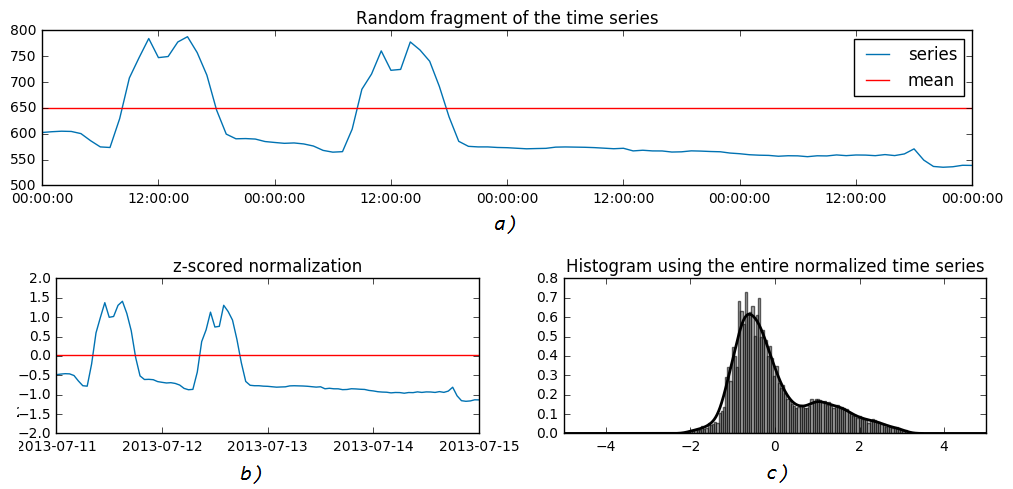
\includegraphics[scale=0.55]{Figures/histogram.jpg}
  \caption{ \textit{a)} Extract of the time series. \textit{ b)} Its corresponding z-score normalization. \textit{c)} Histogram of the entire z-score normalized time series. }
  \label{fig:histogram}
\end{figure}     

Since the underlying distribution of the time series is not a Gaussian distribution, it could be an error to use breakpoints that are defined for a Gaussian distribution. In other words, instead of using the cut-off points (i.e. breakpoints) that are specified in the original SAX approach \cite{lin2003symbolic, keogh2005hot, lin2007experiencing}, we suggest estimate the Probability Density Function (pdf) of the time series, and then, calculating the breakpoints that divide this function in similar areas. Figure \ref{fig:pdf_estimated} shows the pdf of the time series with the corresponding breakpoints.         


\begin{figure}[h!]
  \vspace{0.5em} %better style
  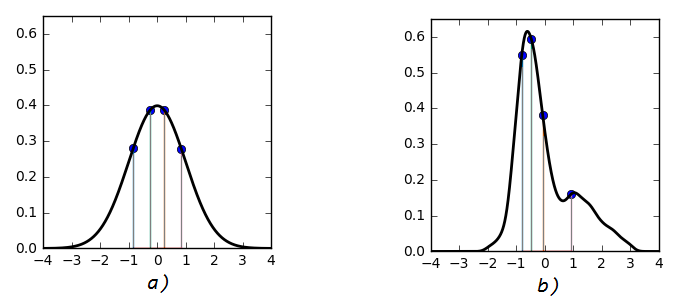
\includegraphics[scale=0.7]{Figures/pdf_estimated.jpg}
  \caption{ \textit{a)} Gaussian distribution divided in 5 equitable areas using the corresponding breakpoints $\beta = [-0.84, -0.25, 0.25, 0.84]$ for $A={a,b,c,d,e}$. \textit{ b)} Estimated pdf of the $CO_2$ level time series divided in 5 equitable areas using the corresponding breakpoints $\beta = [-0.81, -0.47, -0.07, 0.94]$ for $A={a,b,c,d,e}$.}
  \label{fig:pdf_estimated}
\end{figure} 

We think that if DayFilter approach uses customized breakpoints that are fixed according to the actual distribution of the time series, then the results would improve significantly. This can be a motivation for new research. Finally, the results for variables: Temperature for room 101 and Humidity for room 101 are included in Annex \ref{tab:SAXvsGaHMM_all}. We observe almost the same results for the rest of the variables.     

\section{Comments from building specialists}
\label{comments}
The presented thesis was exposed to building control system specialists of Synergy BTC AG\footnote{Dimitrios Gyalistras and Carina Sagerschnig}. Several topics were discussed in reference to the proposed models. Here we list the most important comments:

\begin{itemize}
\item The approach is very interesting, in fact the combination of the \textit{GaHMM profile} with the hierarchical agglomerative clustering provides in a glance the difference between motif profiles and discord profiles. Therefore, the proposed approach assist very well to designers in spotting potential anomalies in the building. There was an agreement in the sense that this approach provides a direct feedback to the stakeholders. 

\item Regarding the practical application of atypical profiles detection that was explained in section \ref{sec:pract_app}. Experts propose for a future study, the evaluation of the detection of atypical profiles using the \textit{GaHMM profile} and HAC approach. For this purpose the ground truth of the process is needed. At the end of this evaluation, the experts expect important indicators like the false positives and false negative rates, and a metric indicator for reliability. 

  
\item Experts agree with our conclusions on the clustering quality of our proposed method on finding cluster profiles. 
When the experts looked at the motif and discord profiles, they asked the question of how much it is going to cost to achieve a 'perfect' performance of the building (i.e. going from discord profiles to motif profiles)? It could be that the price of this optimization task is very expensive and could be difficult to justify. 


\item Other topics discussed with the experts were: What if the proposed approach is used with critical variables? Variables that must be directly controlled with controller devices (bottom part of the building control). It seems that there is great potential to exploit our proposed approach in this domain.
      
\item Money is an important aspect to consider. One possible application which the experts foresee as having a good chance of return on investment, is applying the proposed approach for selling energy to a grid by using renewable energies. Control devices could detect the ideal times to sell energy and thus benefit from this opportunity.   
   

\item Experts believe if the user awareness increases about the dynamics of building, people would be empowered to demand comfort enhancement, lower energy consumption or any other aspect of interest to the user. Our approach could assist the user in this purpose. The experts recommend that if an application is developed for this purpose, the interaction must be easy and fast (only a couple of clicks) due to the lack of interest that could be presented by the occupant after initial use.


\item Since we show that the profile clusters change across seasons and years, experts recommend rerunning the training process at least every four months. This will guarantee an update on all the daily profiles. Additionally, they recommended a yearly evaluation of the patterns to see if there are abrupt changes in the patterns in the building. 

\end{itemize}
    


During the discussion period, the experts shared their personal experiences where they pointed out that our approach might be interesting in the distant future, because currently, the building industry is more focused on practical applications, where the cost/benefit return is evident. Additionally, there is not much interest in optimizing the performance of buildings already constructed since it increases the implementation price of the building. Nevertheless, they do not discredit the use of the proposed approach in other domains where the fine control is important (i.e. building control system). For more practical purposes, our approach can be used over variables that belong to the bottom part process of the building (i.e. building control process) rather than the output variables (i.e. $CO_2$, room temperature, and others). In other aspects, from the point of view of the experts, the \textit{GaHMM profile} model might be more powerful and robust if the model considered multivariate samples similar as it was done for \textit{GaHMM seasonal and interactional} model. In this way the information of other variables (e.g. status of control devices 1/0) makes the model more integral and robust. In short, we received a positive feedback from the experts, and their guidance is relevant for future work.   